\makeatletter\let\ifGm@compatii\relax\makeatother
% Problemas con el paquete geometry se solucionan con la anterior
% sentencia. 18/5/2015
\documentclass[8pt]{beamer}

\usepackage{../IyA.estilo}

%\usepackage{xmpmulti}

\usepackage{animate}

%\usepackage{media9}

%-----------------Titulo y autores

\title{Cap\'itulo 5 \\
	Instrumentos Girosc\'opicos}
\subtitle{C\'atedra de Instrumentos y Avi\'onica}
\author{ Ing. Jorge Garcia}
\institute{
	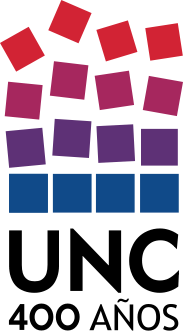
\includegraphics[height=1.5cm]{../imagenes/logos/400-anios} \hspace{3mm}	
	
\includegraphics[height=1cm]{../imagenes/logos/logoUNC} \hspace{1mm}	
	
\includegraphics[height=1cm]{../imagenes/logos/fcefyn} \hspace{1mm}	
	
\includegraphics[height=1cm]{../imagenes/logos/dpto-aero-logo}
	\\
%	Departamento de Aeron\'autica \\
%	Facultad de Ciencias Exactas, F\'isicas y Naturales \\
%	Universidad Nacional de C\'ordoba
	}
\date{A\~no 2019}

%----------------------------------CONTENIDO------------------
% Cap�tulo 5. Instrumentos girosc�picos
% 5.1.      Propiedades girosc�picas aplicadas al instrumental aeron�utico de a bordo.
% 5.2.      Indicadores de virajes, neum�ticos, de CC y CA .
% 5.3.      Indicadores de actitud en dos ejes con gir�scopo integrado, y remoto.
% 5.4.      Magnetismo terrestre, br�jula, gir�scopo direccional libre.
% 5.5.      Comp�s girosc�pico auto-corregido, indicador con gir�scopo integrado, y remoto.
% 5.6.      Central girosc�pica para la indicaci�n de actitud en tres ejes y toda actitud.
% 5.7.      Gir�scopo LASER

\begin{document}

%----------- titlepage -----------%
\begin{frame}[plain]
  \titlepage
\end{frame}

%OK
% 5.1.      Propiedades giroscópicas aplicadas al instrumental aeronáutico de a bordo.
% Version 2019

\section{Propiedades del gir\'oscopo}
\label{sec:propiedades.giroscopo}

\begin{frame}{Un poco de historia...}
  
  \begin{columns}
    \begin{column}{0.3\textwidth}
      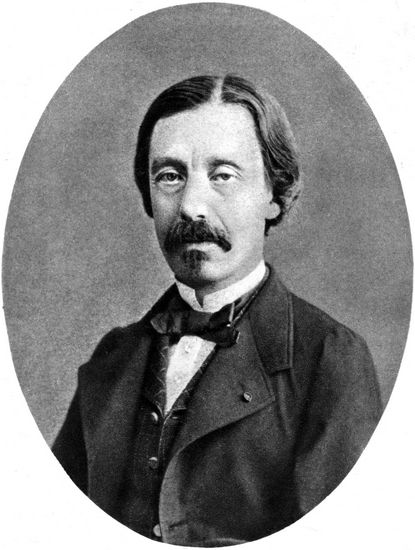
\includegraphics[width=0.7\linewidth]{05.instrumentos.giroscopicos.imagenes/05.01.movimientos/foucault.jpg}

      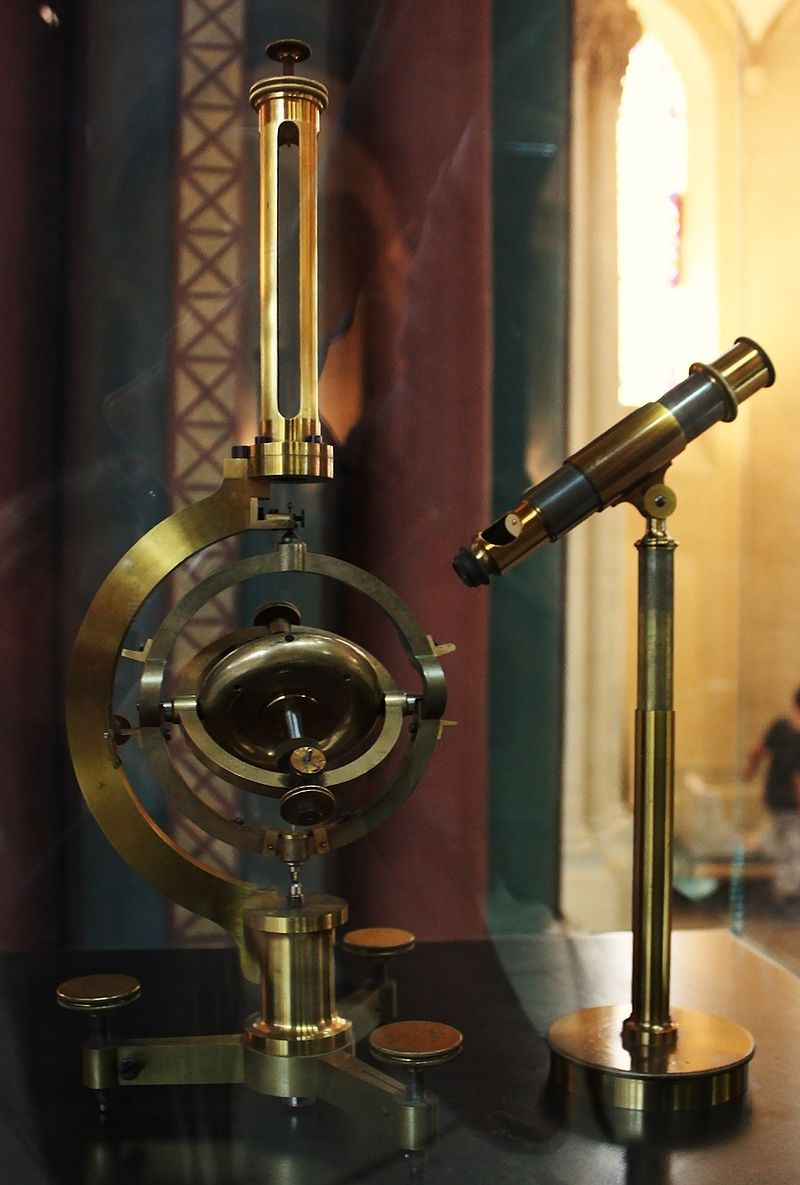
\includegraphics[width=0.7\linewidth]{05.instrumentos.giroscopicos.imagenes/05.01.movimientos/foucault_giroscopo_wiki.jpg}\\
      {\tiny Fuente: Wikipedia}
    \end{column}
    \begin{column}{0.7\textwidth}{\small

  \begin{block}{Etimolog\'ia}
    Gir\'oscopo proviene del griego,
	{\it gyros}: rotaci\'on y {\it skopein}: vista/
  \end{block}

      \begin{exampleblock}{Desarrollo del gir\'oscopo}
        Bernard Le\'on Foucault (1819-1868) invent\'o el gir\'oscopo
        en 1852 y le permiti\'o observar el giro del planeta Tierra.
        Mont\'o una masa rotatoria en un soporte de Cardano para un
        experimento que demostrara la rotaci\'on de la Tierra.  Aunque
        ya hab\'ia demostrado la rotaci\'on de este cuerpo con el
        p\'endulo que lleva su nombre, no comprend\'ia por qu\'e la
        velocidad de rotaci\'on del mismo resultaba m\'as lenta que la
        velocidad de rotaci\'on de la Tierra por un factor
        $\sin{\lambda}$, donde $\lambda$ representa la latitud donde
        se encuentra el p\'endulo.  Por lo anterior, Foucault se di\'o
        cuenta que necesitaba otro aparato para demostrar la
        rotaci\'on de la Tierra de forma m\'as simple y utiliz\'o los
        trabajos del astr\'onomo alem\'an Johann Bohnenberger.
      \end{exampleblock}
	}
    \end{column}
  \end{columns}
  
\end{frame}

\begin{frame}{El gir\'oscopo}

      \begin{columns}
        \begin{column}{0.2\textwidth} \centering

% \animategraphics[loop,width=\linewidth]{10}{05.instrumentos.giroscopicos.imagenes/05.01.movimientos/05.01.giroscopo.animado/giroscopo_animado-}{0}{59}


% \animategraphics[loop,width=\linewidth]{10}{05.instrumentos.giroscopicos.imagenes/05.01.movimientos/05.01.gimbal/gimbal-}{0}{99}

          
        \end{column}
      \begin{column}{0.8\textwidth}
      Un gir\'oscopo consiste en una masa rotante, con forma de rueda, 
	cuyo eje se sujeta a una armaz\'on o cuna (gimbal) 
	interior y \'esta a otra cuna exterior. Este sistema se encuentra libre de rotar en el espacio.

      El gir\'oscopo posee las siguientes propiedades:
      \begin{enumerate}
      \item {\bf Rigidez:} es la que permite que rote siempre en el mismo plano y se opone a cualquier momento
	 que tienda a cambiarlo.
      \item {\bf Precesi\'on:} consiste en la variaci\'on angular del plano de rotaci\'on bajo el influjo 
      de la aplicaci\'on de un momento. Su valor es proporcional a la intensidad del momento aplicado e 
      inversamente proporcional al momento de inercia y momento cin\'etico del rotor.
      \end{enumerate}
    \end{column}
    \end{columns}

	\vspace{0.3cm}
% {\tiny Animaci\'on de un conjunto de tres ejes. Fuente: Lars H. Rohwedder (User:RokerHRO) - Trabajo propio,
%  Dominio p\'ublico, \url{https://es.wikipedia.org/wiki/Suspensi\%C3\%B3n_card\%C3\%A1n#/media/Archivo:Rotating_gimbal-xyz.gif}
% }

%      {\tiny Imagen Suspensi\'on Cardan. Fuente: De Lars H. Rohwedder (User:RokerHRO) - Trabajo propio, 
%      Dominio p\'ublico, \url{https://commons.wikimedia.org/w/index.php?curid=1352775}}

  \href{https://www.youtube.com/watch?v=JnKloSdUJLo}{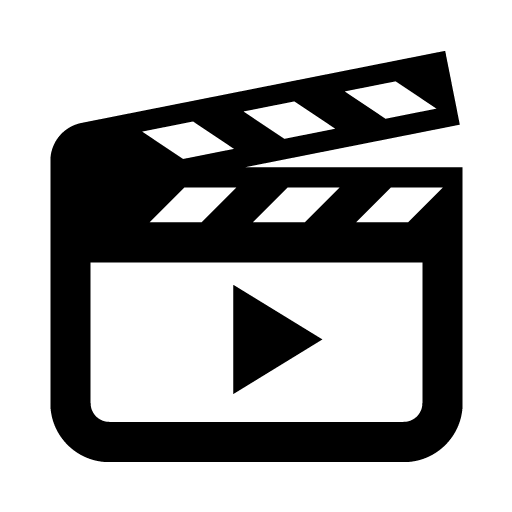
\includegraphics[width=0.1\textwidth]{05.IyA.imagenes/Video.png}}\,Instrumentos girosc\'opicos

\end{frame}

%----------------------Aplicaciones giroscopo
\begin{frame}{Aplicaciones gir\'oscopo}
  \begin{itemize}
  \item Gir\'oscopos libres
    \begin{itemize}
    \item Ejemplo: sistemas inerciales
    \end{itemize}
  \item Gir\'oscopos de desplazamiento
    \begin{itemize}
    \item Dos (2) grados de libertad
    \item Detecta desplazamientos angulares
    \item Utililiza la propiedad de rigidez
    \item Como referencia direccional se emplea uno de eje horizontal
    \item Como referencia en cabeceo y alabeo se emplea uno de eje vertical
    \item Ejemplos: horizonte artificial, comp\'as girosc\'opico
    \end{itemize}
  \item Gir\'oscopos de velocidad
    \begin{itemize}
    \item Un (1) grado de libertad
    \item Detecta velocidades angulares
    \item utiliza la propiedad de precesi\'on
    \item Ejemplo: indicador de giro y viraje
    \end{itemize}

  \end{itemize}
\end{frame}

\begin{frame}{Accionamiento del gir\'oscopo}

  \begin{itemize}
  \item
    \href{https://www.youtube.com/watch?v=q2Zgvxn4rSA}{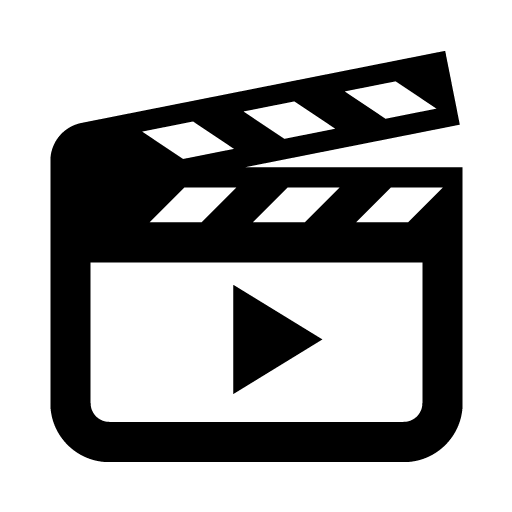
\includegraphics[width=0.1\textwidth]{05.IyA.imagenes/Video.png}}\,
    Gir\'oscopo neum\'atico

  \item     \href{https://www.youtube.com/watch?v=FYSHEhksBjk}{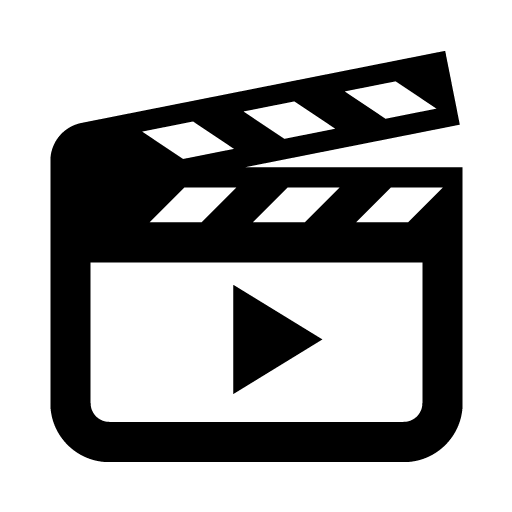
\includegraphics[width=0.1\textwidth]{05.IyA.imagenes/Video.png}}\, 
 \href{https://www.youtube.com/watch?v=VycrS3VYjeM}{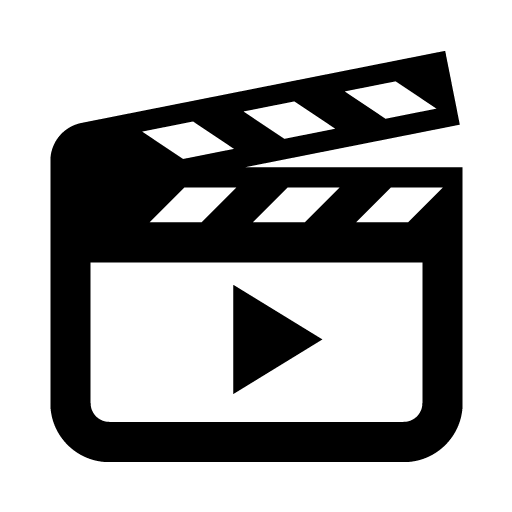
\includegraphics[width=0.1\textwidth]{05.IyA.imagenes/Video.png}}
\, Gir\'oscopo el\'ectrico

\item \href{https://www.youtube.com/watch?v=8IYkisyOZvs}{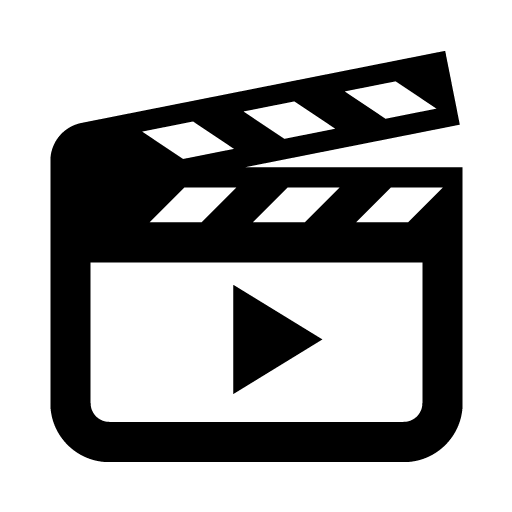
\includegraphics[width=0.1\textwidth]{05.IyA.imagenes/Video.png}}\, Gir\'oscopo laser

\item \href{https://www.youtube.com/watch?v=z62CxCSRMjY}{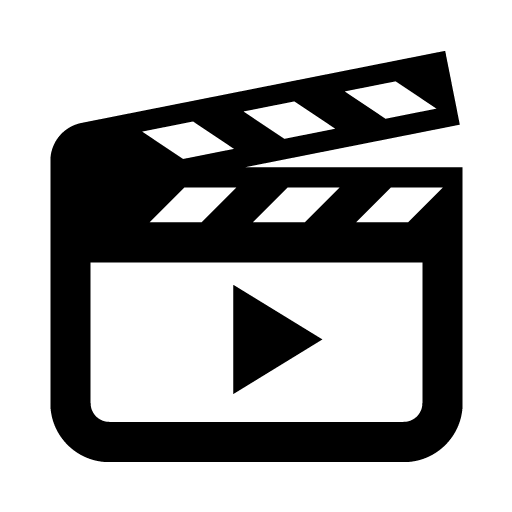
\includegraphics[width=0.1\textwidth]{05.IyA.imagenes/Video.png}}\, Gir\'oscopo de fibra \'optica

  \end{itemize}

\end{frame}




%OK
% 5.2.      Indicadores de virajes, neumáticos, de CC y CA .
% Version 2019

\section{Indicadores de virajes, neum\'aticos, de C.C. y C.A.}
\label{sec:indicadores.de.virajes}

\subsection{Indicadores de virajes}
\label{sec:indicadores.virajes.basico}


\begin{frame}{Indicadores de virajes, neum\'aticos, de CC y CA}

  \begin{block}{Coordinador de giro. Indicador de viraje}

        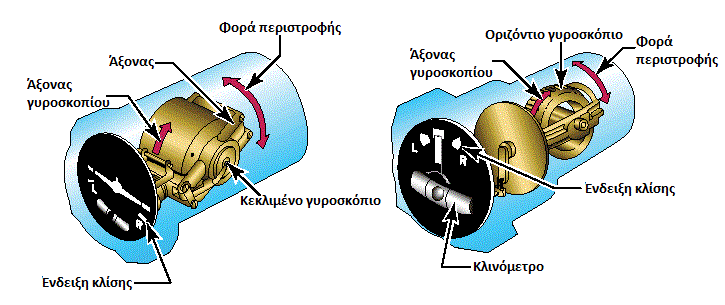
\includegraphics[width=0.95\linewidth]{05.instrumentos.giroscopicos.imagenes/05.02.indicadores.viraje.imagenes/indicador_giro_viraje.png}

      \end{block}

\end{frame}


\begin{frame}{Indicadores de virajes, neum\'aticos, de CC y CA}

  \begin{block}{Indicador de viraje}
    \begin{columns}
      \begin{column}{0.45\textwidth}
        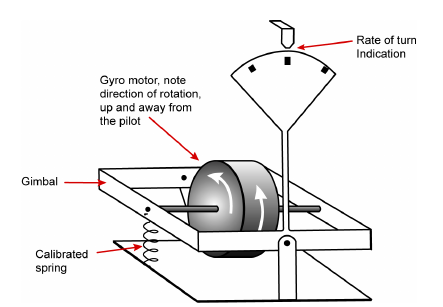
\includegraphics[width=\linewidth]{05.instrumentos.giroscopicos.imagenes/05.02.indicadores.viraje.imagenes/indicador_viraje_01.png}
      \end{column}
      \begin{column}{0.45\textwidth}
        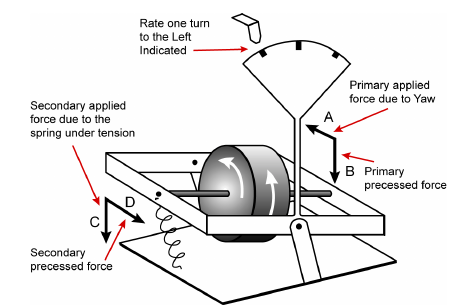
\includegraphics[width=\linewidth]{05.instrumentos.giroscopicos.imagenes/05.02.indicadores.viraje.imagenes/indicador_viraje_02.png}
      \end{column}

    \end{columns}

  \end{block}

\end{frame}

\begin{frame}{Indicadores de virajes, neum\'aticos, de CC y CA}

  \begin{block}{Indicador de viraje}
       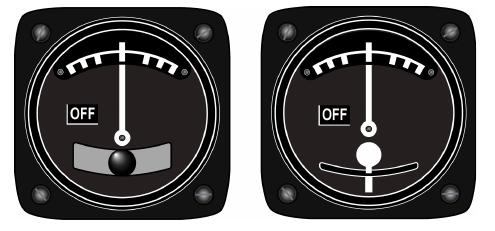
\includegraphics[width=0.85\linewidth]{05.instrumentos.giroscopicos.imagenes/05.02.indicadores.viraje.imagenes/indicador_viraje_03.jpg}
     \end{block}
\end{frame}


\begin{frame}{Indicadores de virajes, neum\'aticos, de CC y CA}

  \begin{block}{Coordinador de giro}
    \begin{columns}
      \begin{column}{0.45\textwidth}
        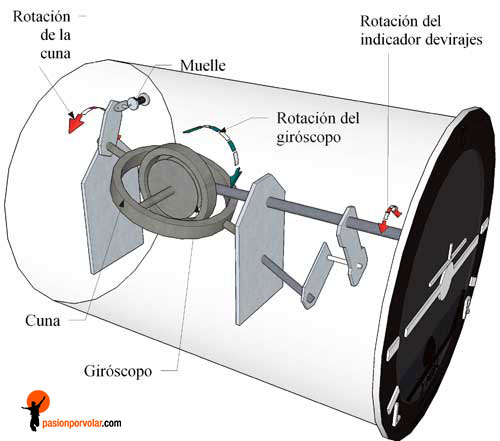
\includegraphics[width=\linewidth]{05.instrumentos.giroscopicos.imagenes/05.02.indicadores.viraje.imagenes/coordinador-de-virajes-1.jpg}
      \end{column}
      \begin{column}{0.45\textwidth}
        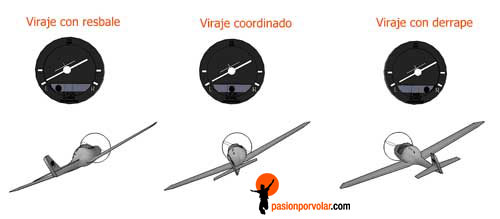
\includegraphics[width=\linewidth]{05.instrumentos.giroscopicos.imagenes/05.02.indicadores.viraje.imagenes/coordinador-de-virajes-2.jpg}

        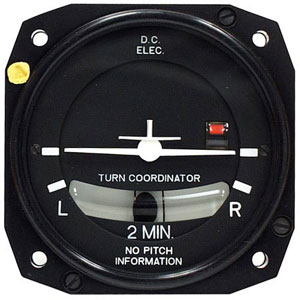
\includegraphics[width=0.4\linewidth]{05.instrumentos.giroscopicos.imagenes/05.02.indicadores.viraje.imagenes/coordinador_viraje.jpg}
      \end{column}

    \end{columns}

  \end{block}

\end{frame}



\begin{frame}{Indicadores de virajes, neum\'aticos, de CC y CA}
  \begin{block}{Coordinador de giro} \centering
       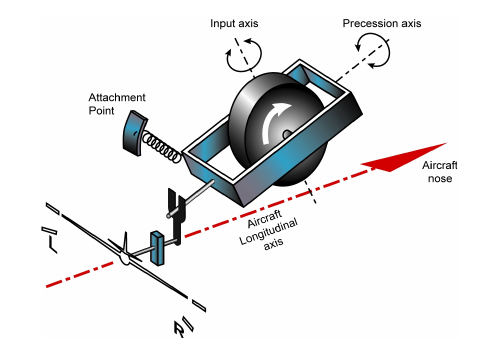
\includegraphics[width=0.65\linewidth]{05.instrumentos.giroscopicos.imagenes/05.02.indicadores.viraje.imagenes/coordinador_viraje_02.png}
     \end{block}

 {\tiny
\href{https://www.youtube.com/watch?v=a4iLtZPp_-8}{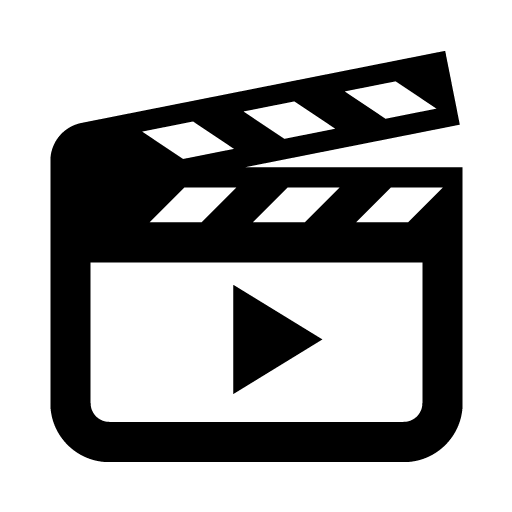
\includegraphics[width=0.1\textwidth]{05.IyA.imagenes/Video.png}}\, Indicador de giro y viraje
 }
\end{frame}
      
\begin{frame}{Indicadores de virajes, neum\'aticos, de CC y CA}

       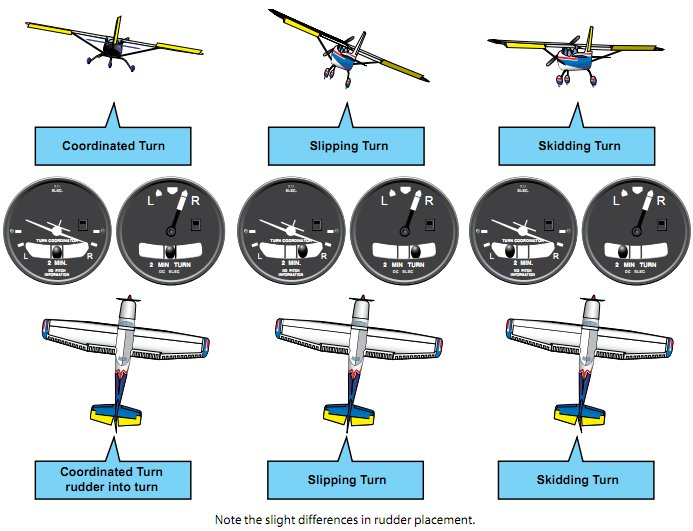
\includegraphics[width=0.75\linewidth]{05.instrumentos.giroscopicos.imagenes/05.02.indicadores.viraje.imagenes/slipping_skidding.jpg}
\end{frame}



%OK
% 5.3.      Indicadores de actitud en dos ejes con giróscopo integrado, y remoto.
% version 2019

\section{Indicadores  de actitud en dos ejes con gir\'oscopo integrado, y remoto}
\label{sec:indicadores.actitud.2.ejes}

\subsection{Indicadores de actitud en dos ejes}
\label{sec:indicadores.actitud.2.ejes.basico}

\begin{frame}

Ver apunte de horizonte artificial
  
\end{frame}



%OK
% 5.4.      Magnetismo terrestre, brújula, giróscopo direccional libre.
% version 2019

\section{Magnetismo terrestre, br\'ujula, gir\'oscopo direccional libre}
\label{sec:magnetismo.terrestre}


\subsection{Magnetismo terrestre}
\label{sec:magnetismo.terrestre.basico}

\begin{frame}{El Campo Magn\'etico Terrestre (CMT)}
  \begin{columns}
    \begin{column}{0.3\textwidth}
  \href{https://www.youtube.com/watch?v=5qDI3O-aKiw}{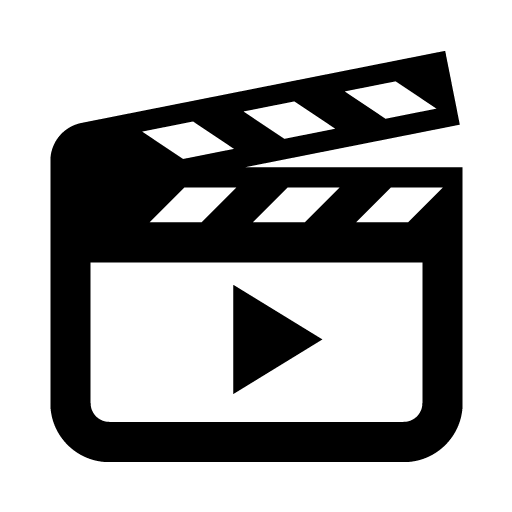
\includegraphics[width=0.15\textwidth]{05.IyA.imagenes/Video.png}}\, Campo magn\'etico terrestre

  \href{https://www.youtube.com/watch?v=UujmN0cZlSw}{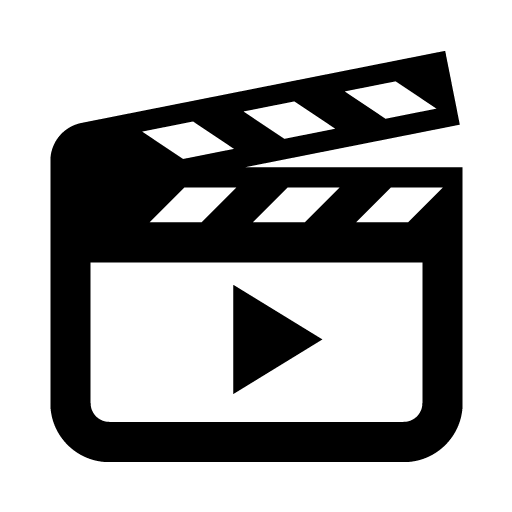
\includegraphics[width=0.15\textwidth]{05.IyA.imagenes/Video.png}}\, Sat\'elites que estudian el campo magn\'etico de la Tierra

    \href{https://www.youtube.com/watch?v=DwshhZq6T8Q}{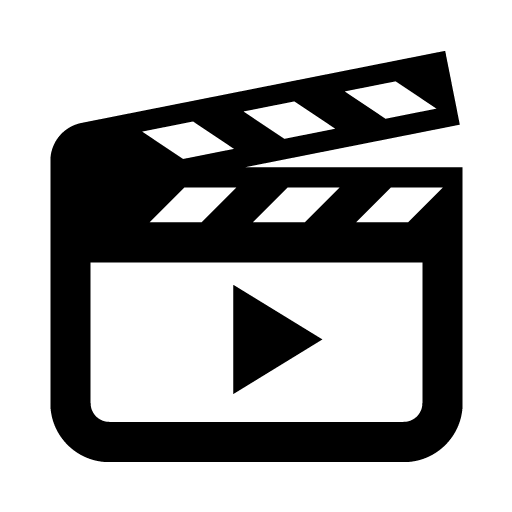
\includegraphics[width=0.15\textwidth]{05.IyA.imagenes/Video.png}}\, Magnetismo terrestre
  \end{column}
  \begin{column}{0.7\textwidth}
    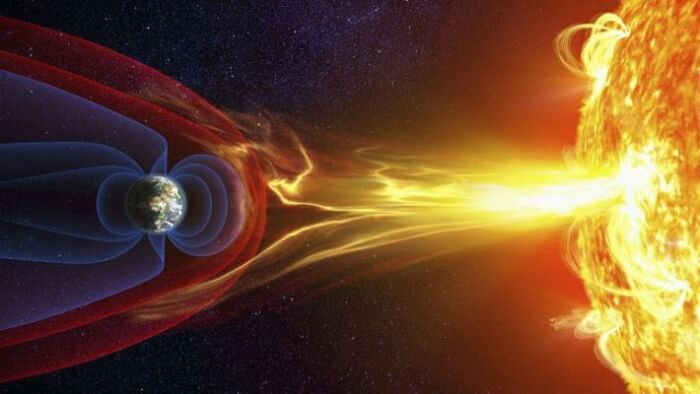
\includegraphics[width=\textwidth]{05.instrumentos.giroscopicos.imagenes/05.04.MagnetismoTerrestre/05-04-campo-magnetico-terrestre.jpg}\vspace{3mm}

    {\tiny Fuente: \url{https://www.capasdelatierra.org/campo-magnetico-magnetosfera/}}
    \end{column}
  \end{columns}
\end{frame}


\begin{frame}

  \begin{exampleblock}{Funci\'on principal del CMT }
    Proteger al planeta Tierra del viento solar
  \end{exampleblock}

  \begin{block}{Caracter\'isticas del CMT}
    \begin{itemize}{\small
    \item El proceso que lo origina se conoce como {\bf geod\'inamo} (hip\'otesis del d\'inamo)
    \item El primero en estudiarlo fue Karl Friedrich Gauss en el siglo XIX
    \item Su intensidad es m\'inima cerca del ecuador y m\'axima cerca de los polos
    \item Es una estructura din\'amica que responde a la actividad del Sol
    \item Los polos geogr\'aficos no coinciden con los magn\'eticos, se mueven en el tiempo
    \item Han existido ``{\it inversiones}'' del campo en la historia del planeta, aproximadamente
      en 20000000 de a\~nos se han invertido cada 200000 - 300000 a\~nos, la \'ultima ocurri\'o
      aproximadamente hace 780000 a\~nos
    \item La interacci\'on con el viento solar produce {\it tormentas magn\'eticas}, algunas
      part\'iculas cargadas quedan atrapadas en la magnet\'osfera y se precipitan a las regiones polares,
      chocando con mol\'eculas de ox\'igeno y nitr\'ogeno, emitiendo luz roja y verde conocidas
      como {\it auroras boreales} en latitud norte y {\it auroras australes} en latitud sur.
}
    \end{itemize}
  \end{block}\vspace{0.3mm}

{\footnotesize
Mayores detalles sobre el CMT pueden encontrarse en 
\href{https://es.gizmodo.com/como-funciona-el-campo-magnetico-de-la-tierra-en-seis-1792481678}{\TextoAzul{C\'omo funciona el campo magn\'etico de la Tierra, en seis espectaculares GIF}}
}

\end{frame}

\begin{frame}
  \begin{columns}
    \begin{column}{0.40\textwidth} \centering
      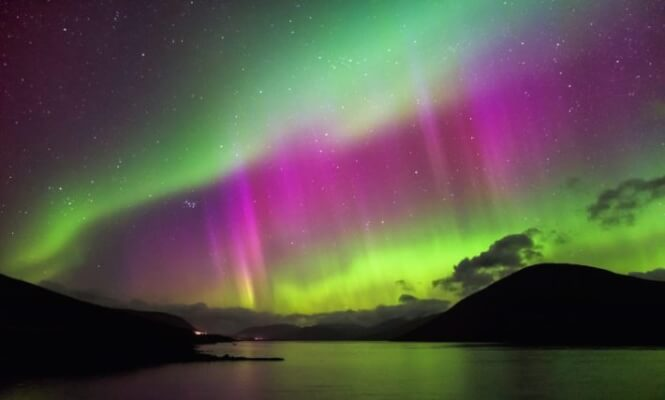
\includegraphics[width=\textwidth]{05.instrumentos.giroscopicos.imagenes/05.04.MagnetismoTerrestre/05-04-auroras.jpg}\vspace{0.3mm}
      Aurora \vspace{0.6mm}

	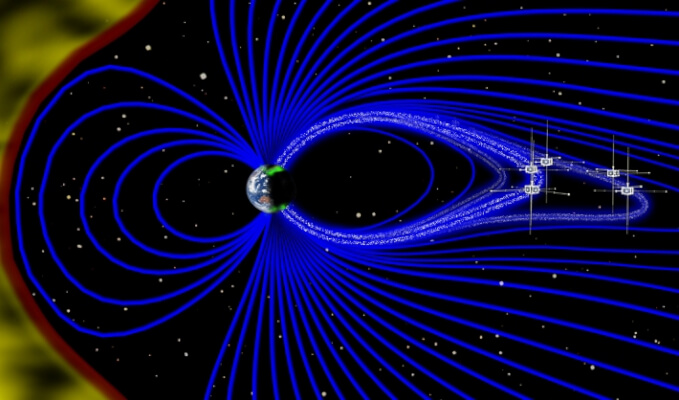
\includegraphics[width=\textwidth]{05.instrumentos.giroscopicos.imagenes/05.04.MagnetismoTerrestre/05-04-cola-del-campo-magnetico.jpeg}\vspace{0.3mm}
      Interacci\'on del CMT con el viento solar \vspace{0.6mm}

\end{column}
    \begin{column}{0.40\textwidth}

      	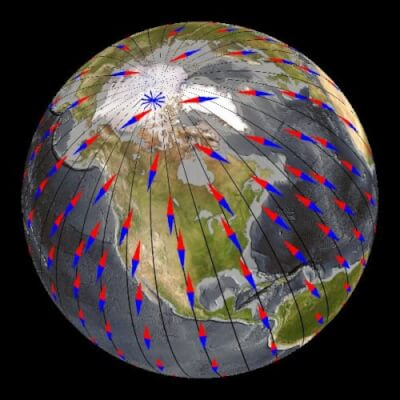
\includegraphics[width=\textwidth]{05.instrumentos.giroscopicos.imagenes/05.04.MagnetismoTerrestre/05-04-polos-de-la-tierra.jpg}
	\end{column}

\end{columns}\vspace{3mm}

    {\tiny Fuente: \url{https://www.capasdelatierra.org/campo-magnetico-magnetosfera/}}

\end{frame}

\begin{frame}
  
  \begin{columns}
    \begin{column}{0.7\textwidth}
  \begin{block}{Propiedades del CMT }{\small
    \begin{itemize}
    \item {\bf Intensidad:} resulta m\'axima en los polos y m\'inima en la zona del ecuador
	con un rango entre 25000 a 65000 nanoTesla (0,25 a 0,65 Gauss). En la actualidad se est\'a
	debilitando con una tasa de 10-15\% en los \'ultimos 150 a\~nos. Su intensidad ha subido y bajado
	en el pasado, siendo las mismas dentro de los valores obtenidos por registros de los campos magn\'eticos
	grabados en rocas.
    \item {\bf Inclinaci\'on:} se inclina hacia el suelo en la zona de los polos magn\'eticos, hasta
	quedar perpendicular a la superficie, y rota progresivamente hasta quedar horizontal al suelo 
	en el ecuador magn\'etico. En un mapa las l\'ineas de igual inclinaci\'on magn\'etica 
	se denominan {\it isoclinas}, del griego {\it isoklines = puntos de la tierra con igual inclinaci\'on
	magn\'etica}
    \item {\bf Declinaci\'on:} 
	En un mapa las l\'ineas de igual declinaci\'on magn\'etica 
	se denominan {\it isogonas}, del griego {\it isogonios = cuerpo geom\'etrico de \'angulos iguales}
    \item {\bf Dipolaridad:} el campo magn\'etico presenta un polo norte y otro sur, que no coinciden
	con los polos geogr\'aficos, y su ubicaci\'on es variable en el tiempo.
    \end{itemize}
  }
\end{block}
\end{column}
\begin{column}{0.3\textwidth}
  \begin{center}
    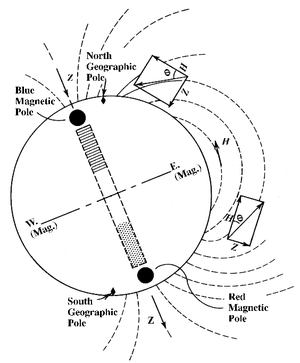
\includegraphics[width=\textwidth]{05.instrumentos.giroscopicos.imagenes/05.04.MagnetismoTerrestre/05-04-desviacion_polos.png}\\
    Inclinaci\'on del CMT
  \end{center}
\end{column}
\end{columns}

\end{frame}

\begin{frame}

  \begin{block}{Variaciones del CMT}{\small
    \begin{itemize}
    \item {\bf Variaciones temporales de corto plazo:} variaciones peri\'odicas en la fuente que genera
	al CMT o de fen\'omenos exteriores.
    \item {\bf Variaciones temporales de largo plazo:} al superar un (1) a\~no terrestre de duraci\'on,
	se las conoce como \TextoRojo{Variaciones Seculares}. Son causadas por dos tipos de procesos que tienen lugar en el n\'ucleo terrestre. El primero est\'a  relacionado con las variaciones del campo principal de un dipolo y opera con escalas de tiempo de cientos o miles de a\~nos. El segundo se relaciona con las variaciones del campo no dipolar, en escalas de tiempo del orden de decenas de anos.
    \item {\bf Inversi\'on de campo:} seg\'un se explic\'o anteriormente
    \end{itemize}
}
  \end{block}
\vspace{0.3mm}
Se puede obtener mucha informaci\'on sobre estos temas y tambi\'en planos actualizados en  \href{https://www.ngdc.noaa.gov/ngdc.html}{\TextoAzul{National Ocean and Atmospheric Administration}}

\end{frame}

\begin{frame}{Mapa Intensidad de CMT}
    
 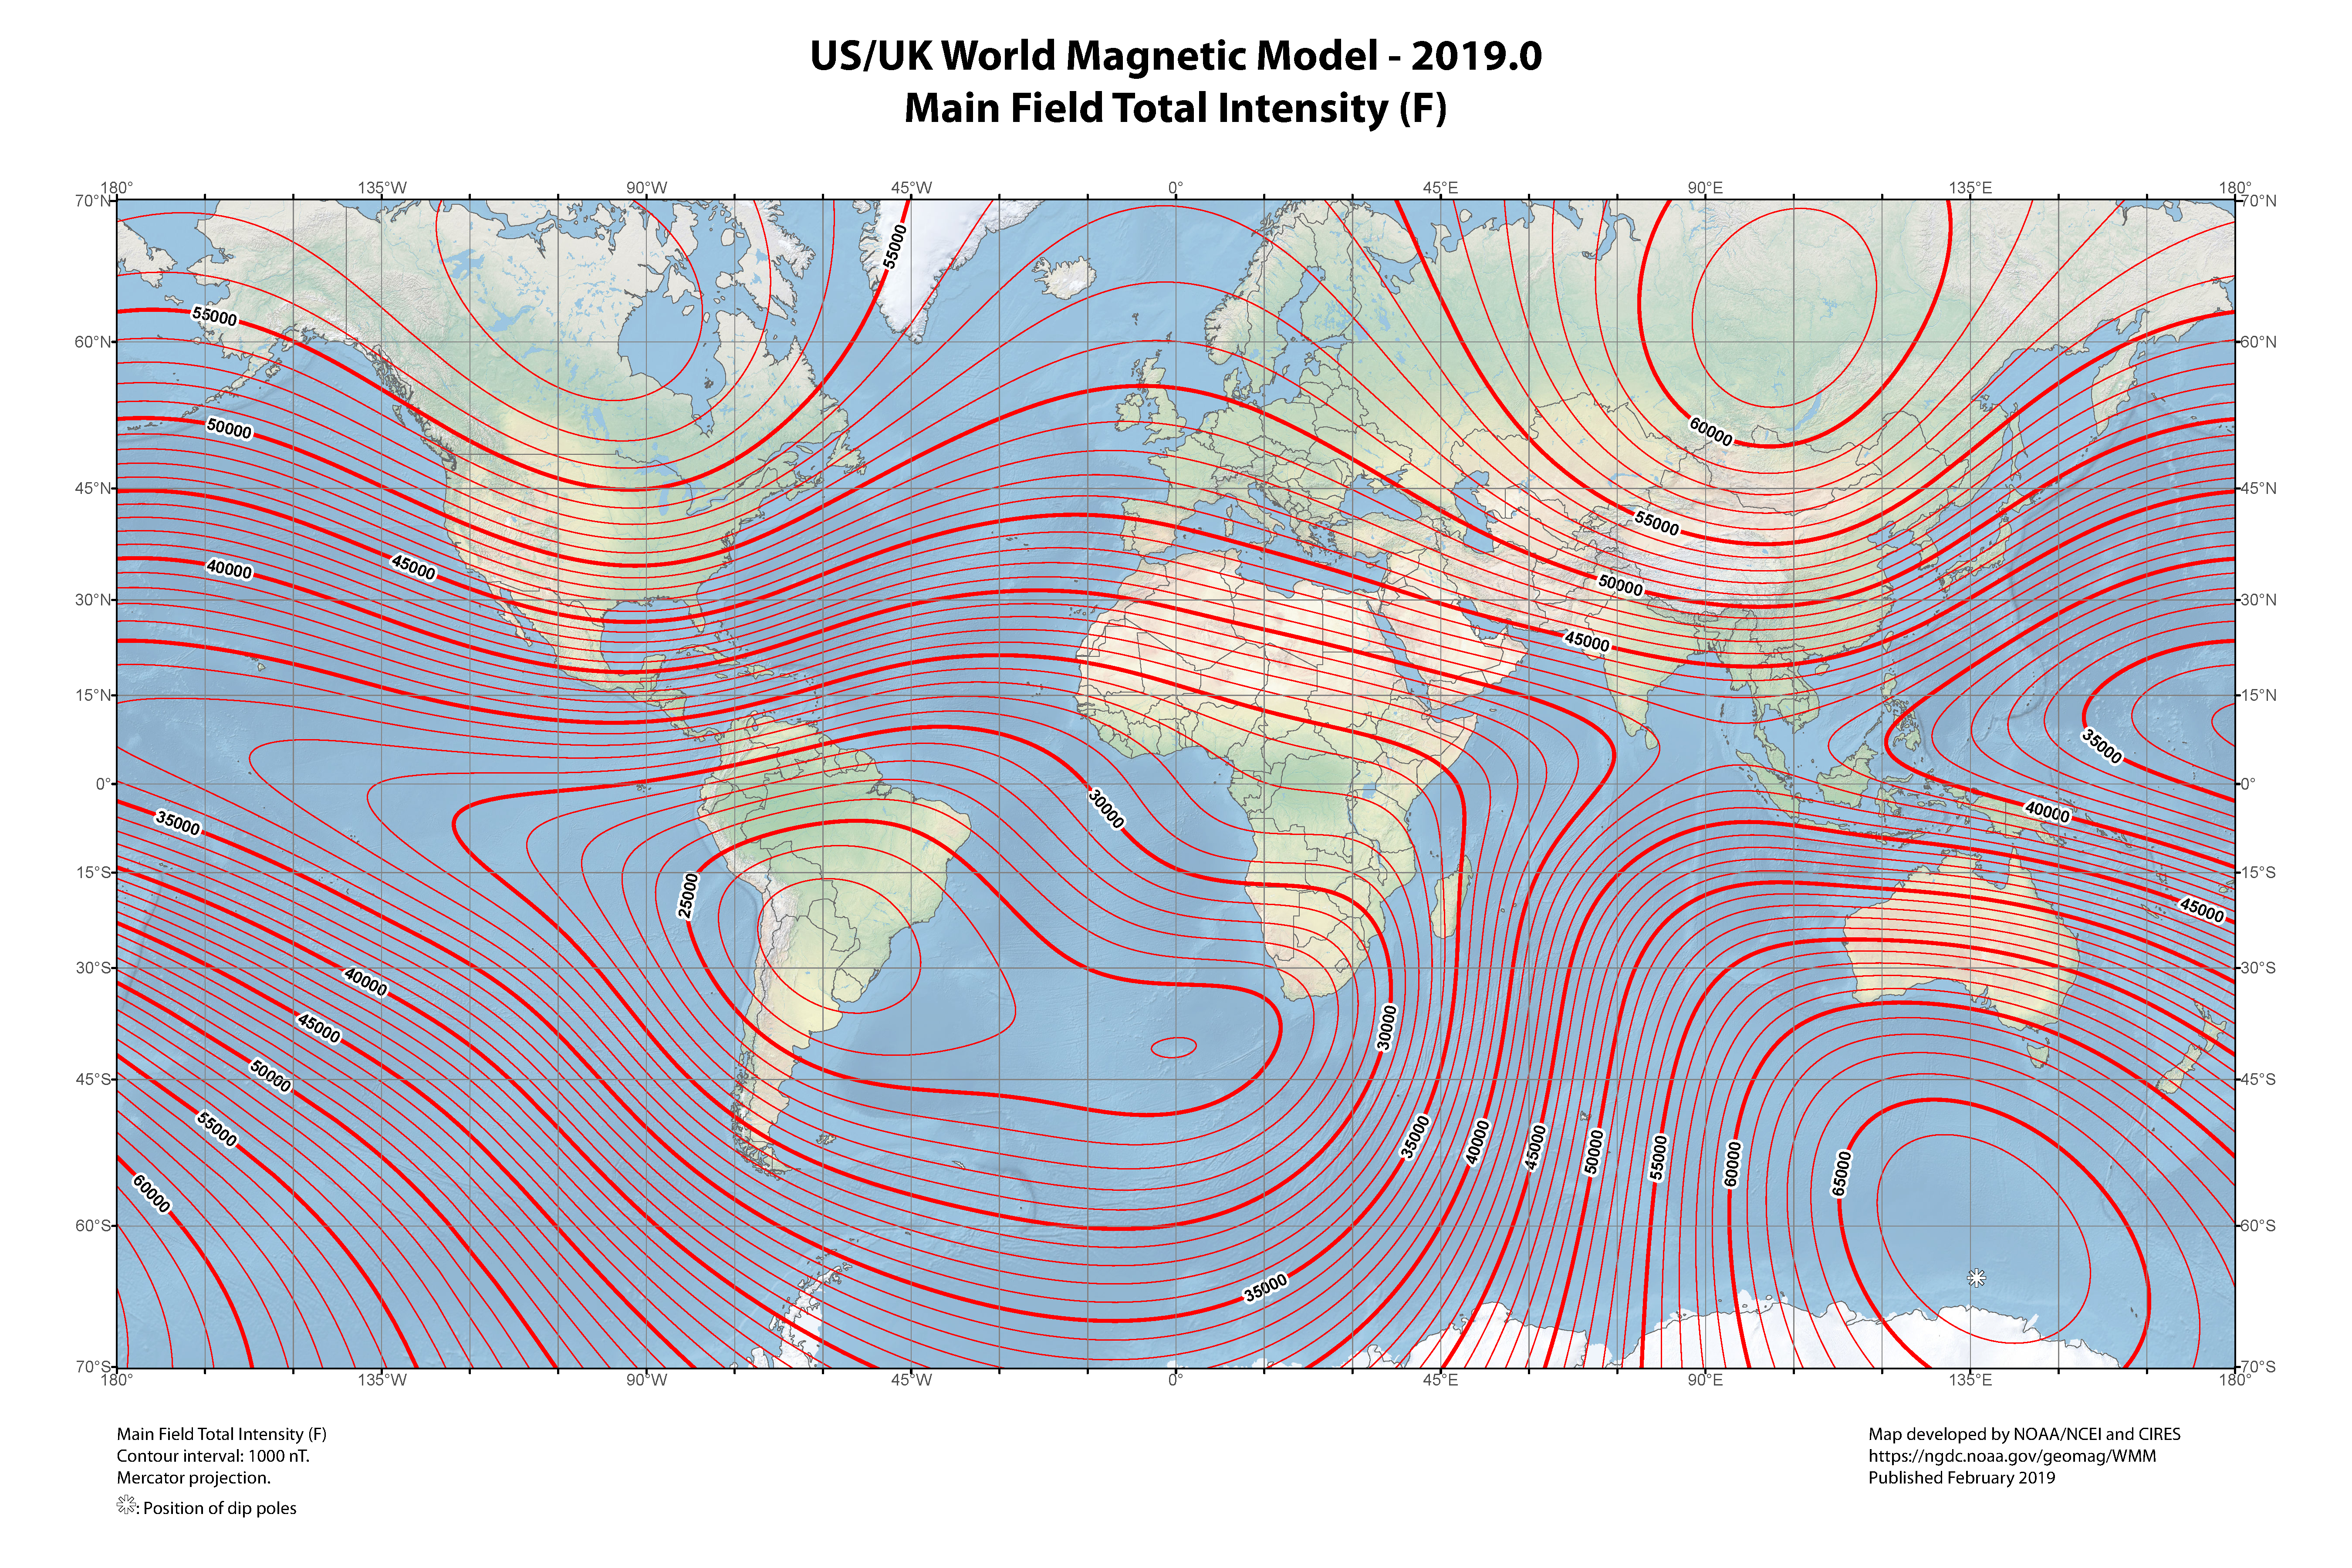
\includegraphics[width=\linewidth]{05.instrumentos.giroscopicos.imagenes/05.04.MagnetismoTerrestre/05-04-mapa_intensidad.pdf}  

\end{frame}

\begin{frame}{L\'ineas Isoclinas}
  
 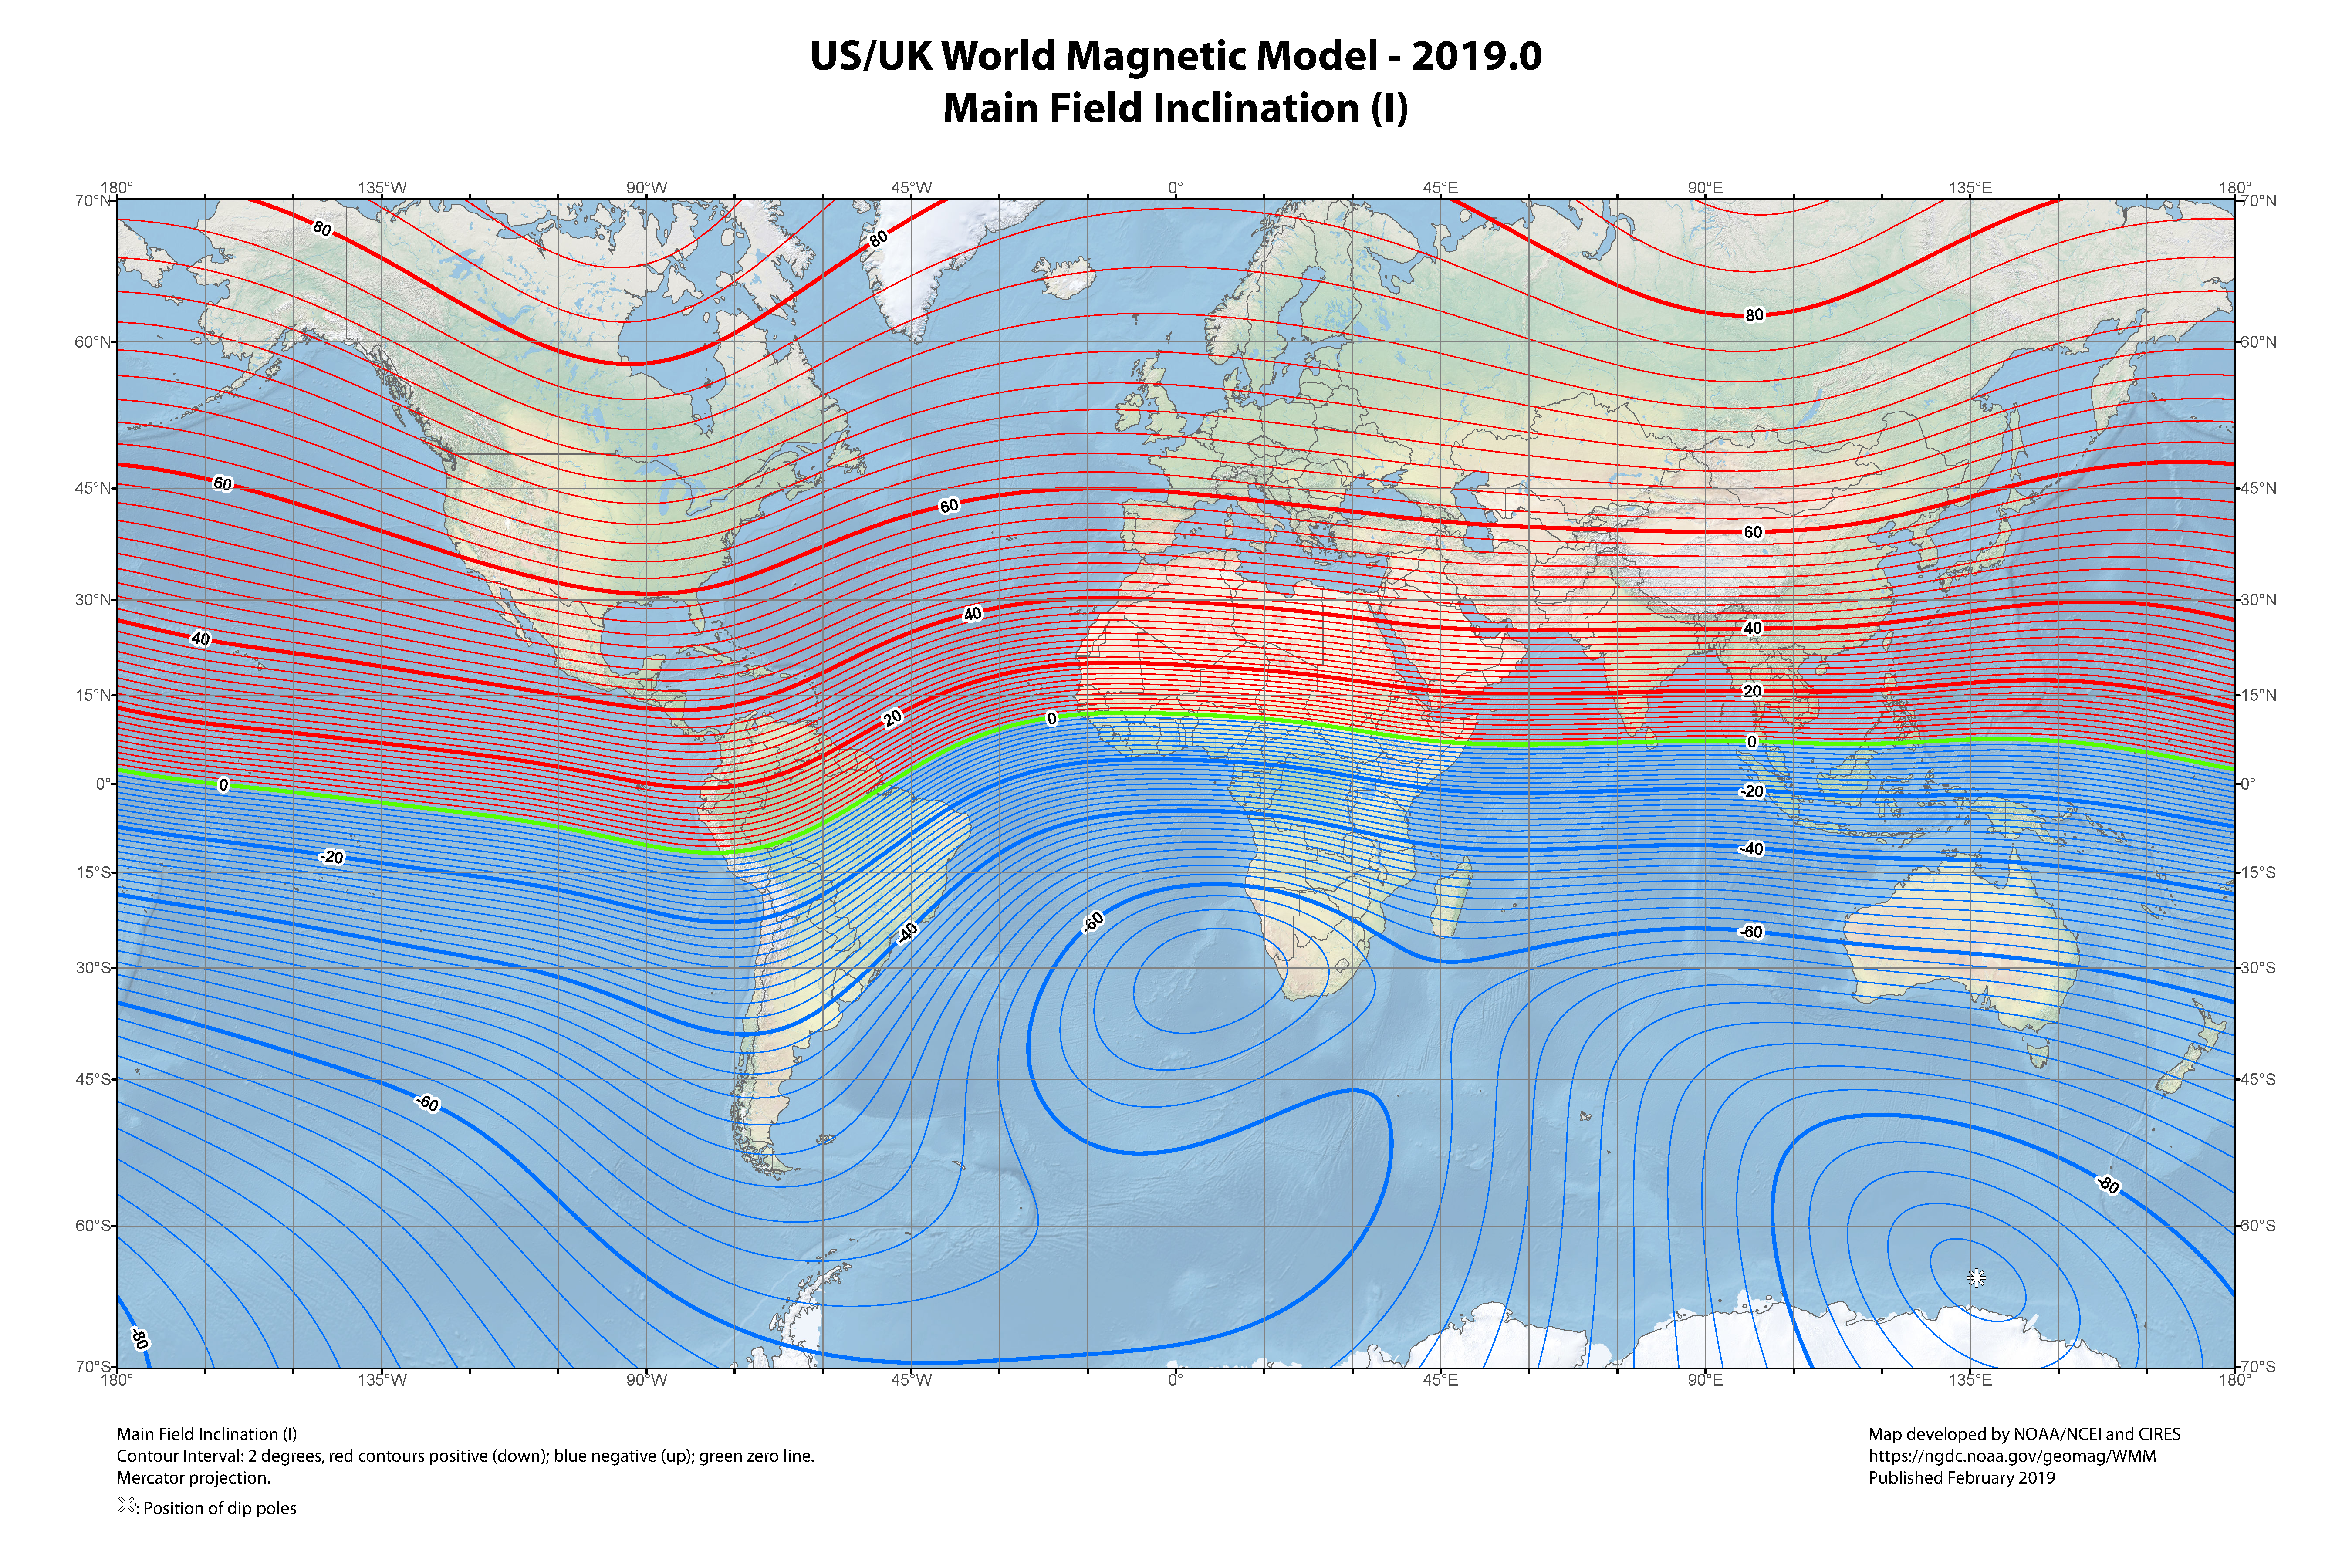
\includegraphics[width=\linewidth]{05.instrumentos.giroscopicos.imagenes/05.04.MagnetismoTerrestre/05-04-mapa_inclinacion.pdf}

\end{frame}

\begin{frame}{L\'ineas Is\'ogonas}
  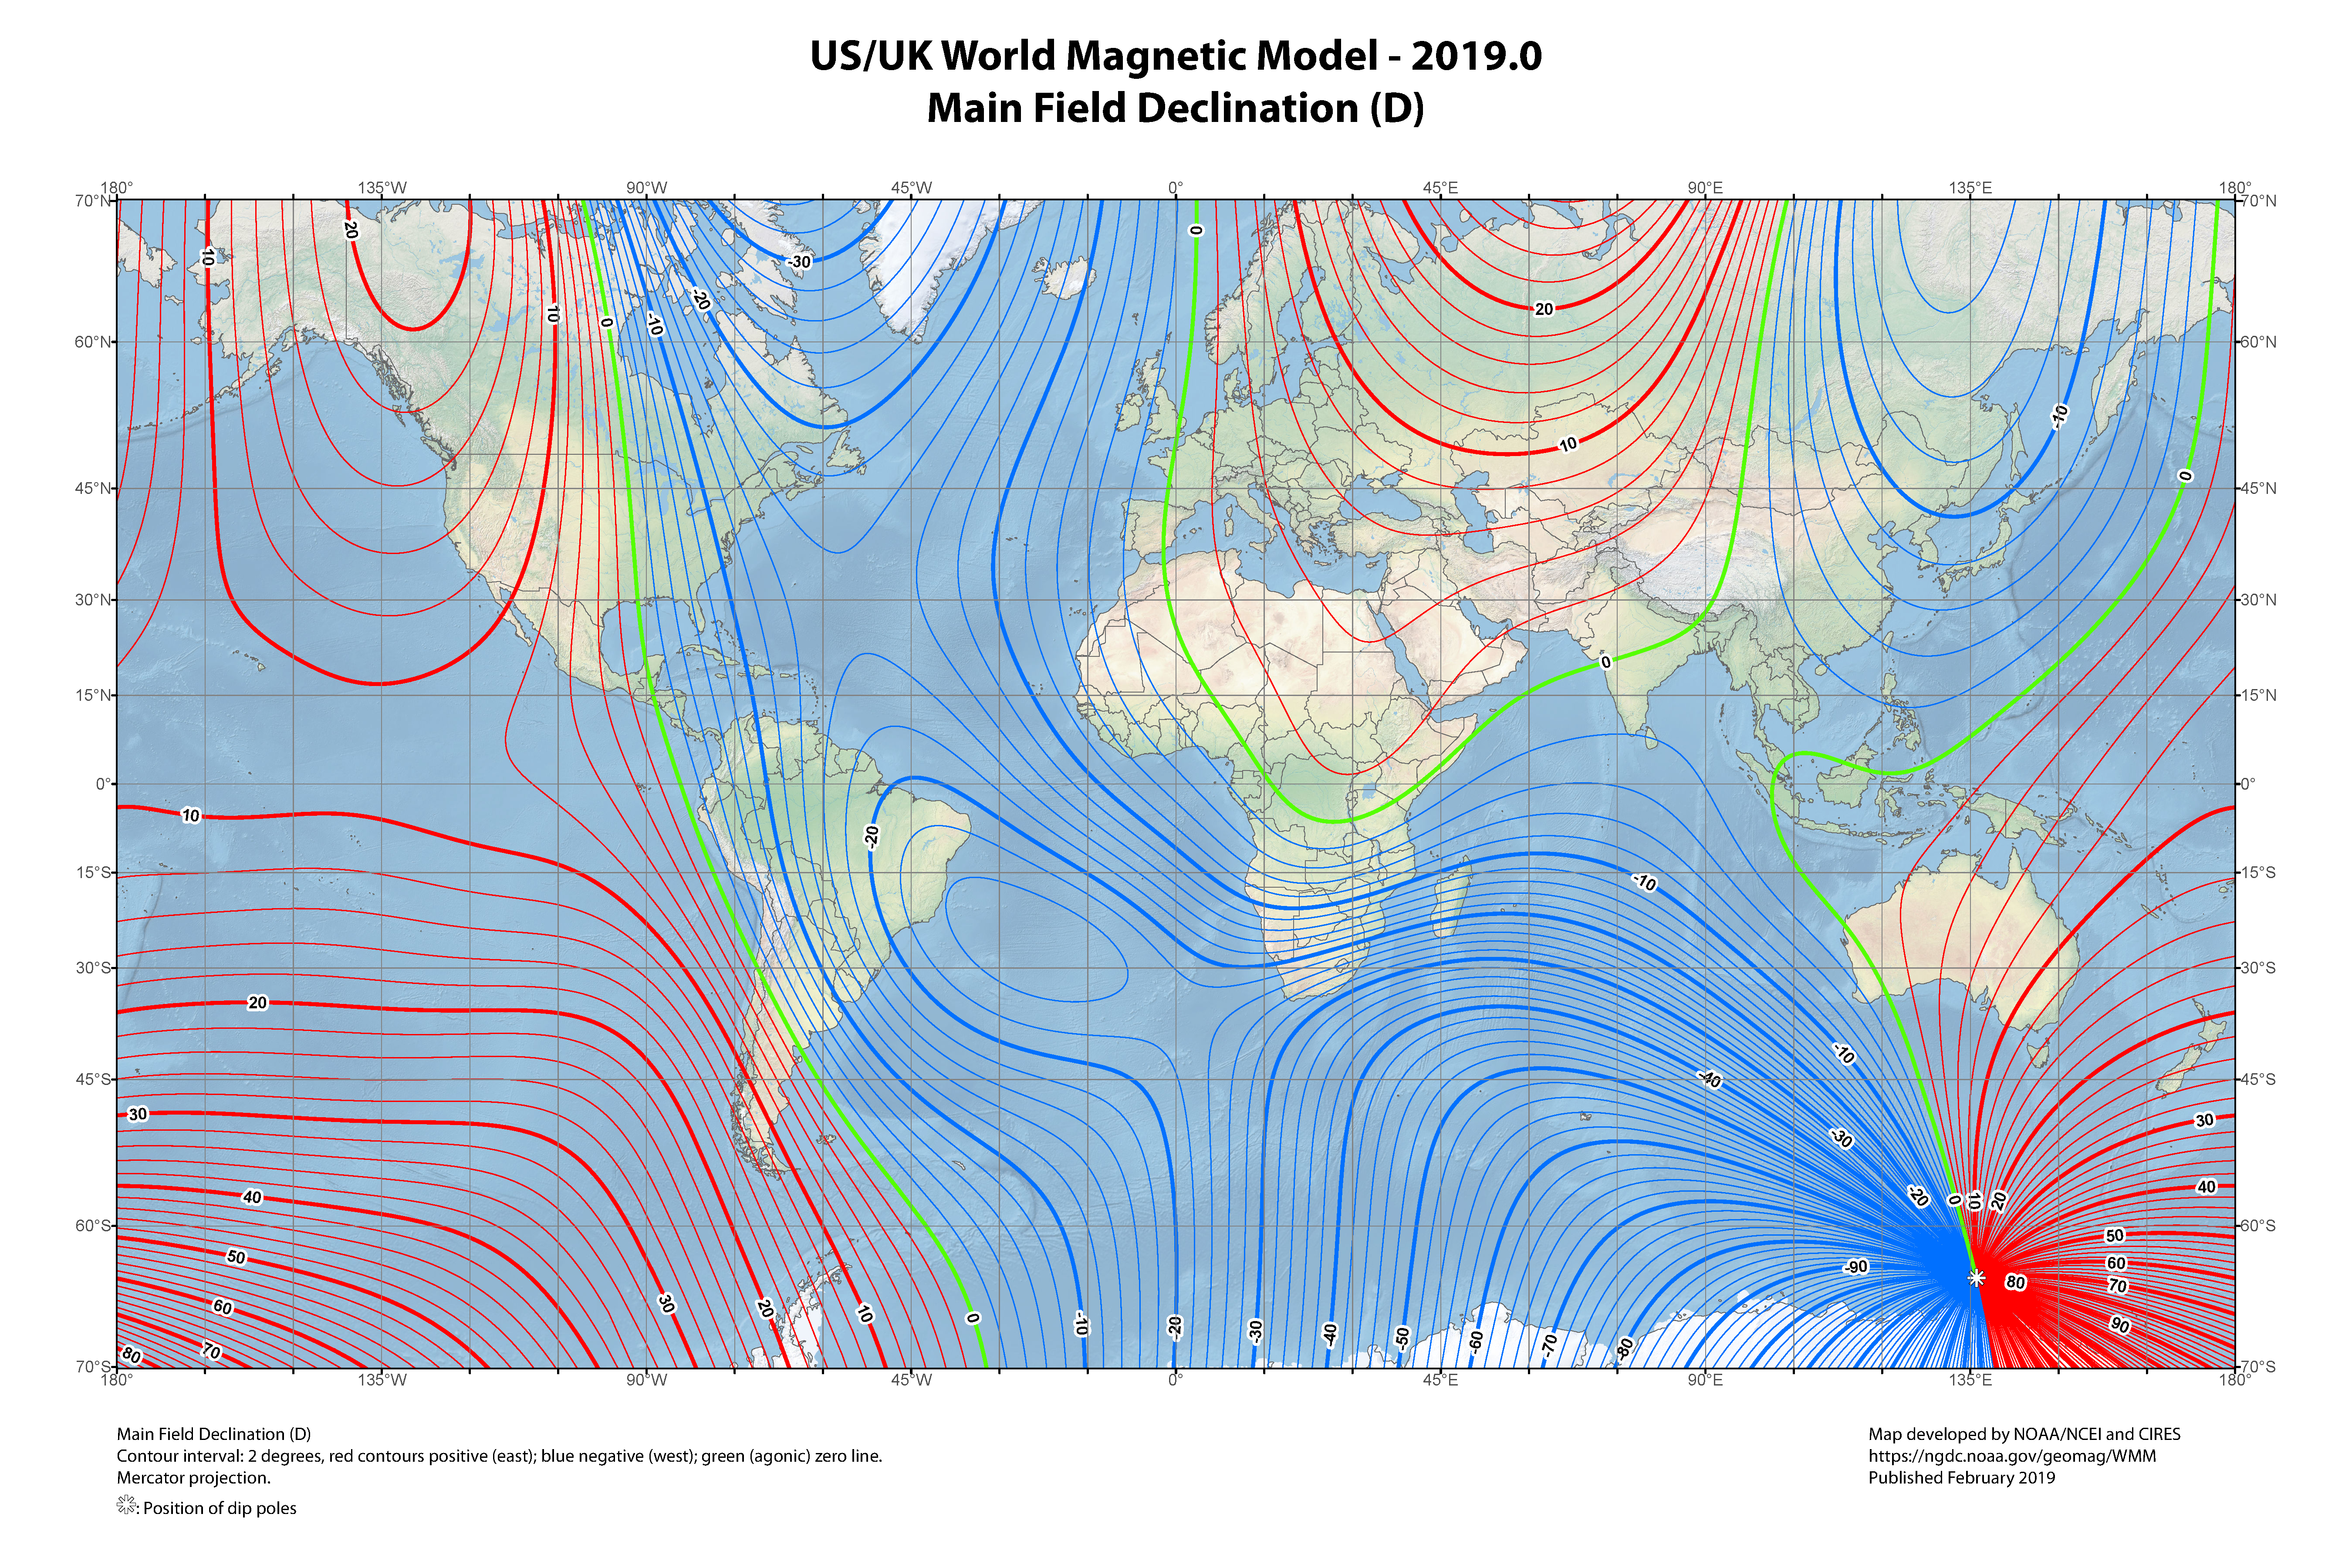
\includegraphics[width=\linewidth]{05.instrumentos.giroscopicos.imagenes/05.04.MagnetismoTerrestre/05-04-mapa_declinacion_2019.pdf}

  {\tiny Fuente: \url{https://www.ngdc.noaa.gov/ngdc.html}
  }
  
\end{frame}

% \begin{frame}{L\'ineas Is\'ogonas}
%   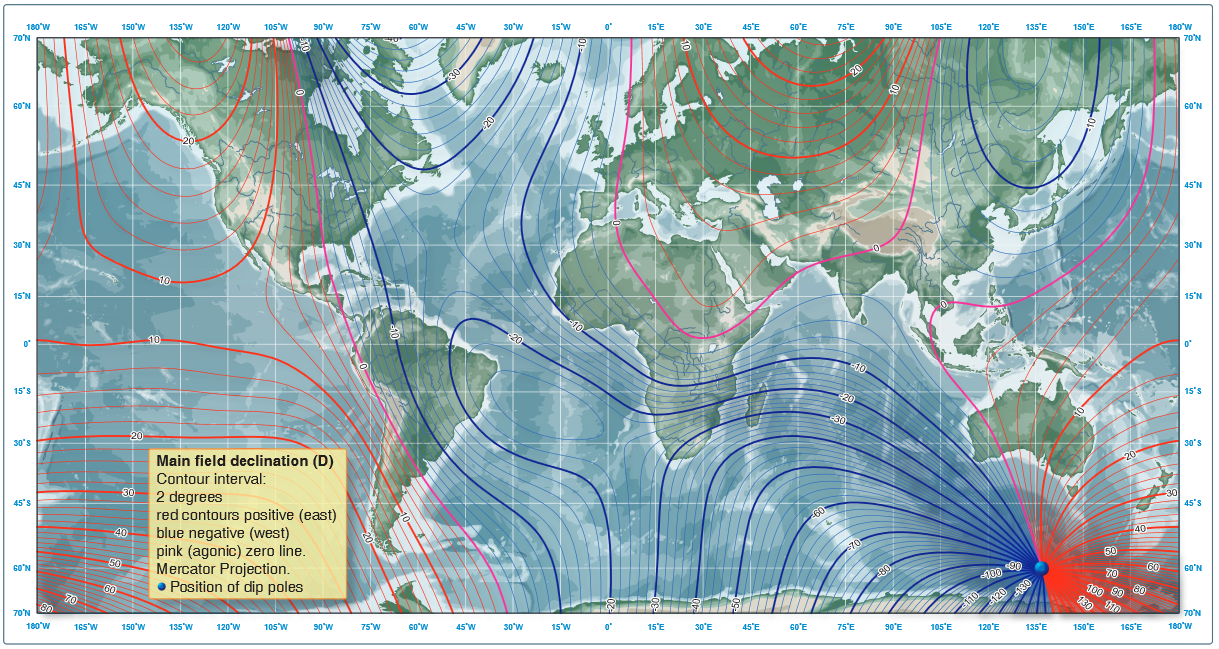
\includegraphics[width=\linewidth]{05.instrumentos.giroscopicos.imagenes/05.04.MagnetismoTerrestre/05-04-isogonic-lines-of-variation.png}

%   {\tiny Fuente: \url{https://www.cfinotebook.net/notebook/avionics-and-instruments/magnetic-compass}
%   }
  
% \end{frame}


\begin{frame}
  
  \begin{block}{Aplicaciones del CMT }
    \begin{itemize}
    \item Los animales vivos pueden detectarlo y lo utilizan para orientarse durante sus migraciones (\TextoVerde{magnetorrecepci\'on})
    \item En la navegaci\'on, mar\'itima o a\'erea, para orientarse desde el siglo XII
    \item Estudio de estructuras geol\'ogicas subterr\'aneas
    \end{itemize}
  \end{block}


\end{frame}

\begin{frame}{Forma constructiva  br\'ujula magn\'etica}

    \begin{center}
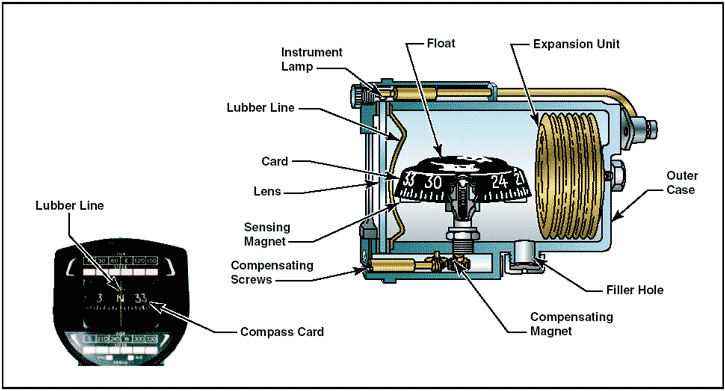
\includegraphics[width=\textwidth]{05.instrumentos.giroscopicos.imagenes/05.04.MagnetismoTerrestre/05-04-brujula_magnetica_construccion.png}
\end{center}

\end{frame}

\begin{frame}{Forma constructiva  br\'ujula magn\'etica}

    \begin{center}
      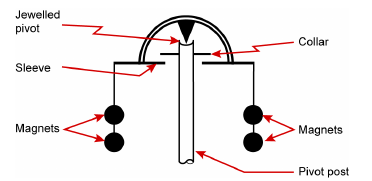
\includegraphics[width=0.56\textwidth]{05.instrumentos.giroscopicos.imagenes/05.04.MagnetismoTerrestre/05-04-brujula_magnetica.png}
      \qquad
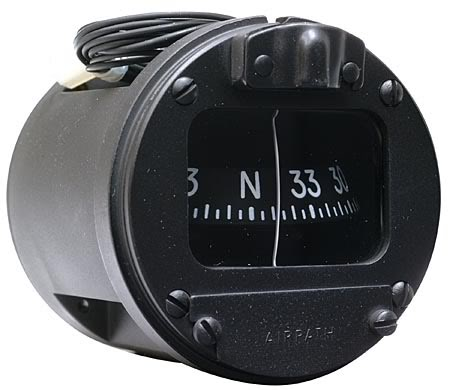
\includegraphics[width=0.35\textwidth]{05.instrumentos.giroscopicos.imagenes/05.04.MagnetismoTerrestre/05-04-MagneticCompass.jpg}      
\end{center}

\begin{block}{Propiedades}

\begin{multicols}{3}
    \begin{itemize}
         \item Horizontabilidad
         \item Sensibilidad
         \item Aperiodicidad
    \end{itemize}
\end{multicols}
\end{block}

\end{frame}

\begin{frame}{  Br\'ujula magn\'etica. Horizontabilidad }

%    \begin{center}
  \begin{columns}

    \begin{column}{0.65\textwidth}
      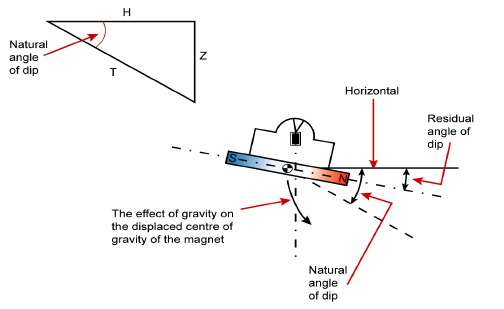
\includegraphics[width=\linewidth]{05.instrumentos.giroscopicos.imagenes/05.04.MagnetismoTerrestre/05-04-brujula_magnetica_inclinacione.png}
    \end{column}
    
    \begin{column}{0.4\textwidth}

    \begin{alertblock}{Requerimiento}
      Resulta escencial que la br\'ujula se mantenga lo m\'as cercano posible al plano horizontal
    \end{alertblock}

    \begin{exampleblock}{Soluci\'on}
      Mediante la forma constructiva y de suspensi\'on en forma de p\'endulo, con su centro de gravedad
      por debajo del punto de suspensi\'on.\\
      El \'angulo residual de inclinaci\'on puede ser $< 3$º
    \end{exampleblock}

    \end{column}
    
  \end{columns}


%    \end{center}

    % It is therefore essential that the compass magnets should lie as close as possible to the horizontal plane

\end{frame}

\begin{frame}{  Br\'ujula magn\'etica. Sensibilidad }

%   Sensitivity is a measure of the ability of the compass magnetic assembly to point accurately
%   towards north.
%   Nothing can be done to increase the strength of the weak terrestrial magnetic field and so it is
% necessary to use several magnets with high pole strengths. The magnetic assembly is made as light as
% possible to reduce friction at the pivot.
% 9.
% The pivot itself normally incorporates a jewelled bearing which is lubricated by the viscous
% fluid which fills the bowl. Being fairly dense the fluid effectively lightens the magnet assembly still
% further, once again reducing friction at the pivot.

  La sensibilidad es una medida de la habilidad del instrumento para indicar con precisi\'on hacia el norte.

  Dado que no puede aumentarse la intensidad del CMT, se utilizan varios imanes de gran intensidad y
  se reduce todo lo posible la fricci\'on en el punto de pivote.
  Este usualmente es una piedra preciosa lubricado por el l\'iquido que contiene el instrumento que, al
  ser cierta densidad, permite una cierta flotaci\'on de la carta, reduciendo la fricci\'on.
  
  \begin{center}
  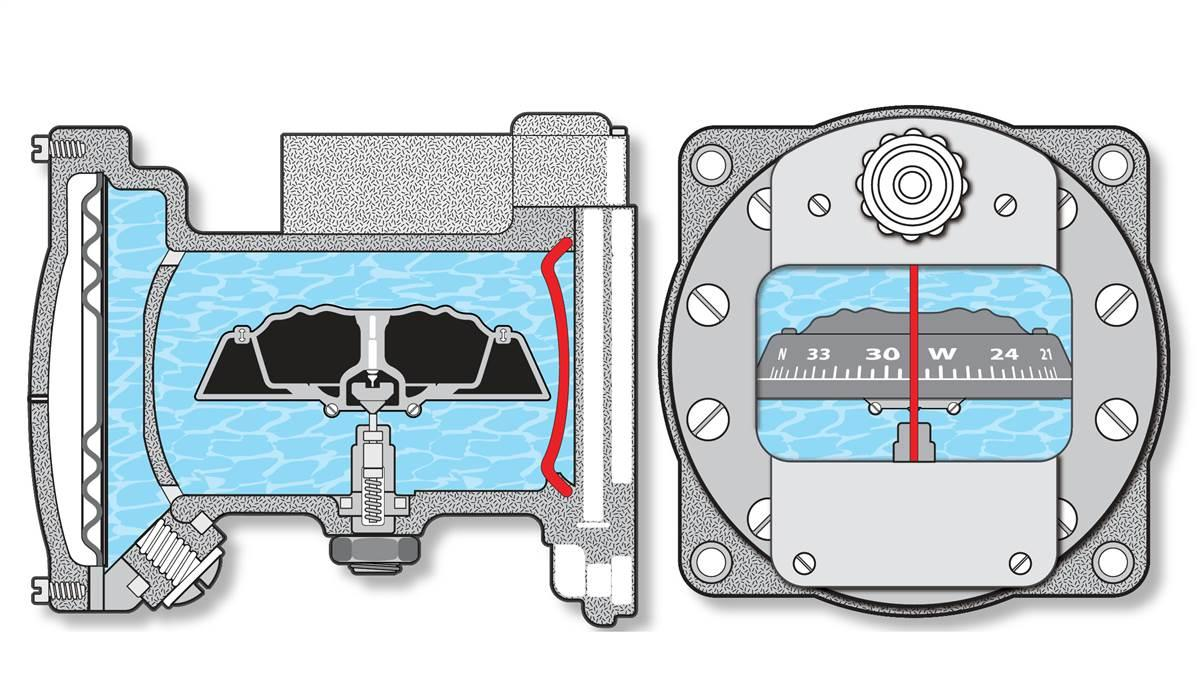
\includegraphics[width=0.7\textwidth]{05.instrumentos.giroscopicos.imagenes/05.04.MagnetismoTerrestre/05-04-1704f_pf_hiw_16x9.jpg}
\end{center}

  
\end{frame}

 \begin{frame}{  Br\'ujula magn\'etica. Aperiodicidad }

 La aperiodicidad se define como la habilidad del sistema para amortiguar r\'apidamente las oscilaciones, apuntando hacia el polo norte magn\'etico, despu\'es de un desplazamiento por maniobras o turbulencias.
  
 Si una br\'ujula magn\'etica no es enteramente aperi\'odica, el efecto es que su indicaci\'on oscila alrededor del norte magn\'etico, llegando a descansar s\'olo lentamente.

 La aperiodicidad se logra utilizando imanes peque\~nos, manteniendo la masa del conjunto oscilante
 cerca de su punto pivote y reduciendo el momento de inercia total. Esto puede lograrse utilizando
 materiales ligeros en la parte m\'ovil y mediante la viscosidad del fluido amortiguante. \'Este
 fluido debe ser transparente y  llenar completamente el interior del instrumento para evitar oscilaciones.
 Para \'esto se provee unas c\'apsulas de expansi\'on debido a efectos de temperatura.

 \end{frame}  

\begin{frame}{Br\'ujula magn\'etica. Distancias de seguridad}

  Uno de los mayores problemas con el comp\'as magn\'etico es que resulta de lectura directa, por lo
  que debe ubicarse en la cabina del piloto y, por lo tanto, se encuentra rodeado por
  equipos que pueden causarle desviaci\'on a su indicaci\'on.

  Por lo anterior, debe estudiarse cuidadosamente la ubicaci\'on del instrumento.

  Como recomendaciones sobre la ubicaci\'on del mismo:

  \begin{itemize}
  \item Cada equipo el\'ectrico o electr\'onico cercano no debe causar una desviaci\'on
    de no mas de 1\grad en el comp\'as. La suma total de los errores de todos los equipos de este
    tipo debe ser menor a 2\grad.
  \item De la misma manera, los cables de conexi\'on de cada equipo, desviaciones $< 1$\grad, para
    todos los cables, $<2$\grad.
  \item La operaci\'on de los equipos en cabina, desviaci\'on $< 1$\grad
  \item Cuando el comp\'as magn\'etico es el instrumento principal para el rumbo, la desviaci\'on
    m\'axima de cualquier rumbo $< 3$\grad.
  \end{itemize}
 
 
 \end{frame}

\begin{frame}{Comp\'as magn\'etico de carta vertical}
  Tambi\'en conocido como tipo E.

  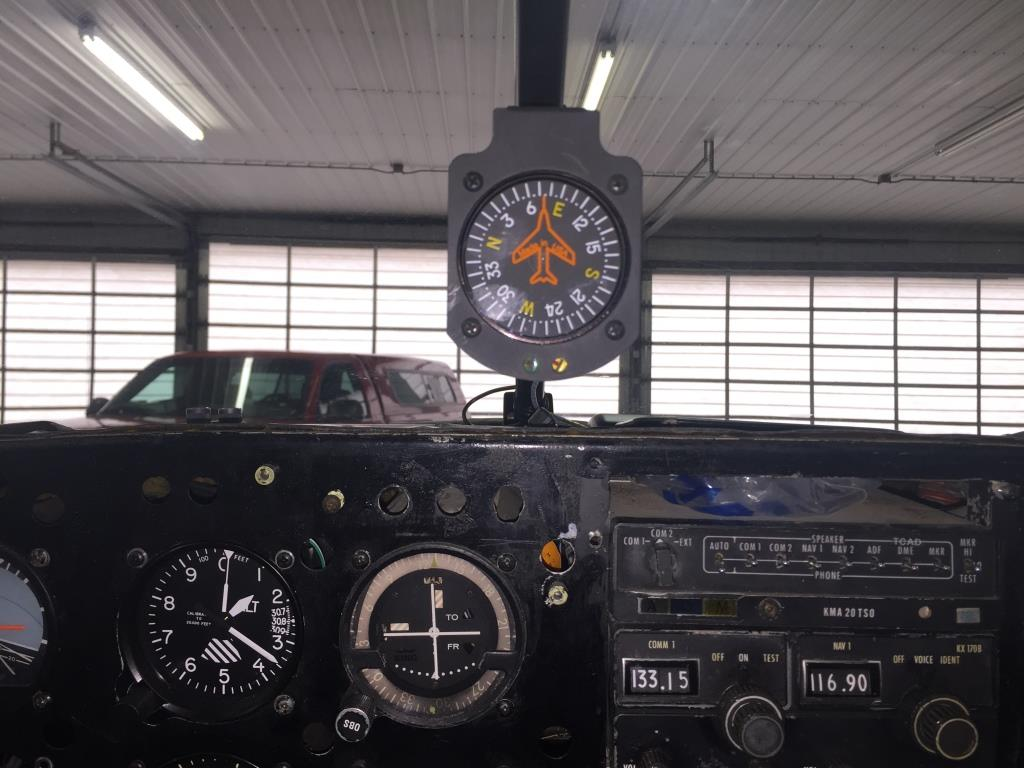
\includegraphics[width=0.35\textwidth]{05.instrumentos.giroscopicos.imagenes/05.04.MagnetismoTerrestre/05-04-IMG_6513.JPG} \hspace{1mm}
      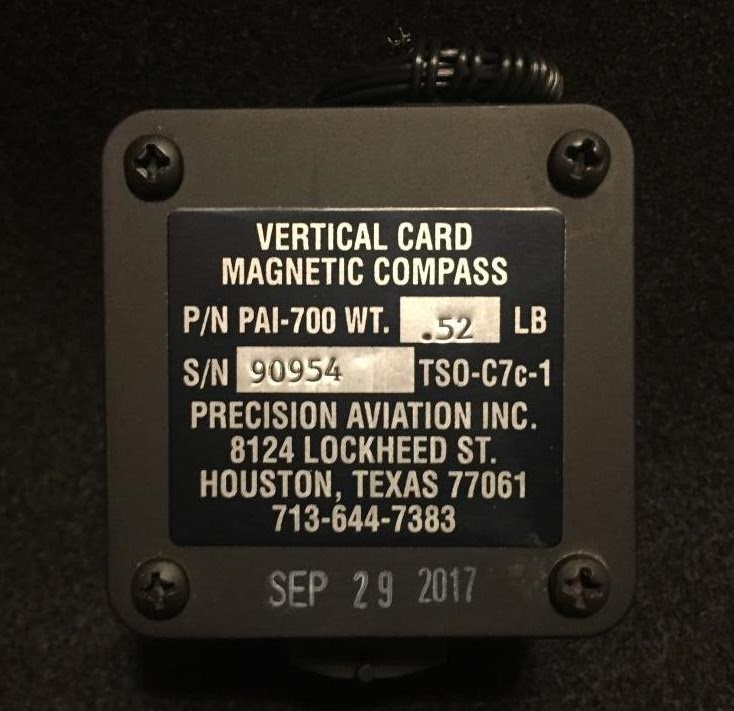
\includegraphics[width=0.25\textwidth]{05.instrumentos.giroscopicos.imagenes/05.04.MagnetismoTerrestre/05-04-IMG_6464.JPG} \hspace{1mm}
      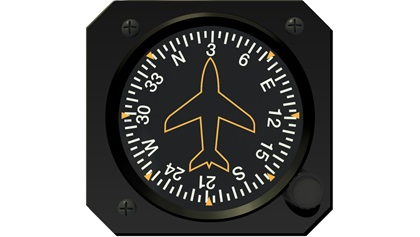
\includegraphics[width=0.45\textwidth]{05.instrumentos.giroscopicos.imagenes/05.04.MagnetismoTerrestre/05-04-VerticalCardCompass.jpg}
      
  {\tiny Fuente: \url{http://n98297.blogspot.com/2017/12/pai-700-compass-installation.html}}
\end{frame}


\begin{frame}

  \begin{alertblock}{Errores  br\'ujula magn\'etica}
    \begin{itemize}
    \item Aceleraci\'on
    \item Giro
    \item Movimiento del l\'iquido
    \end{itemize}
  \end{alertblock}

\end{frame}

\begin{frame}{Errores br\'ujula magn\'etica. Aceleraci\'on}

Debido a la inercia. 

  \begin{center}
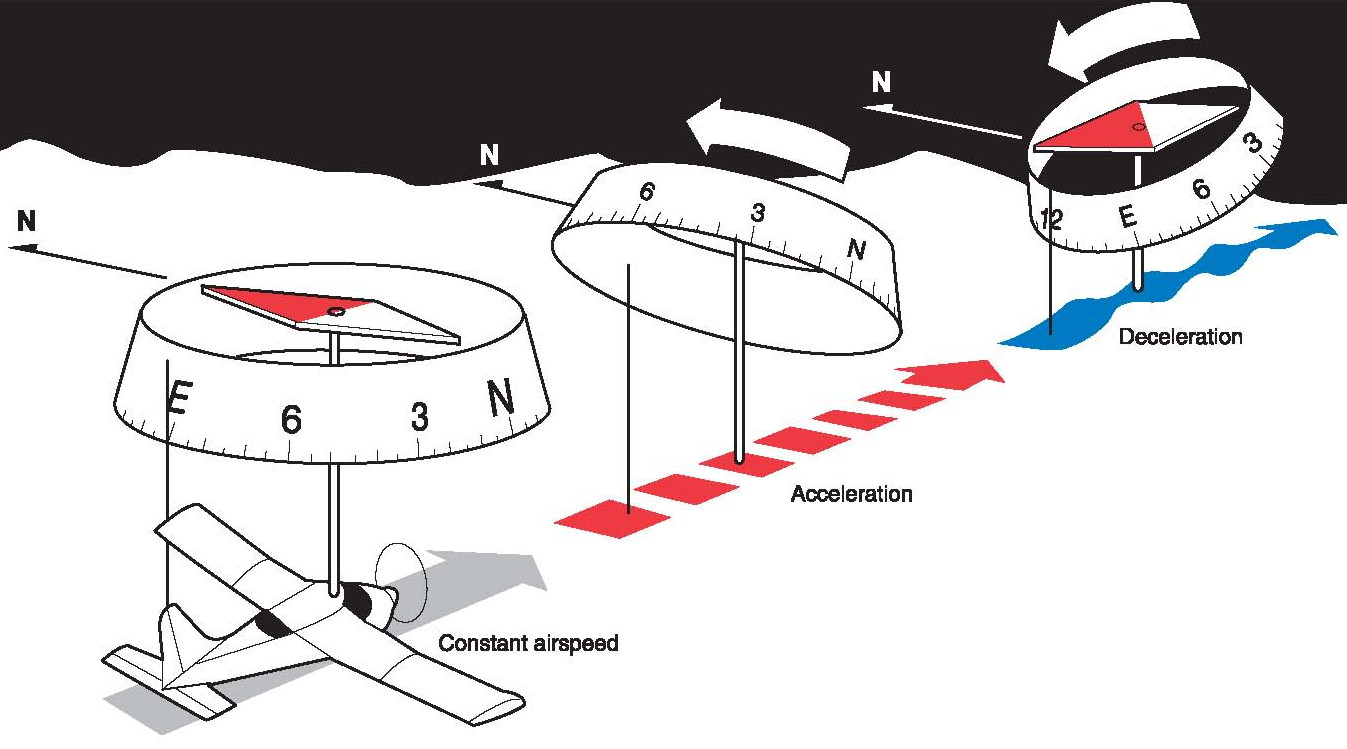
\includegraphics[width=0.80\textwidth]{05.instrumentos.giroscopicos.imagenes/05.04.MagnetismoTerrestre/05-04-brujula_error_aceleracion.jpg}
\end{center}
  
\href{https://www.youtube.com/watch?v=vUz09IpYCuY}{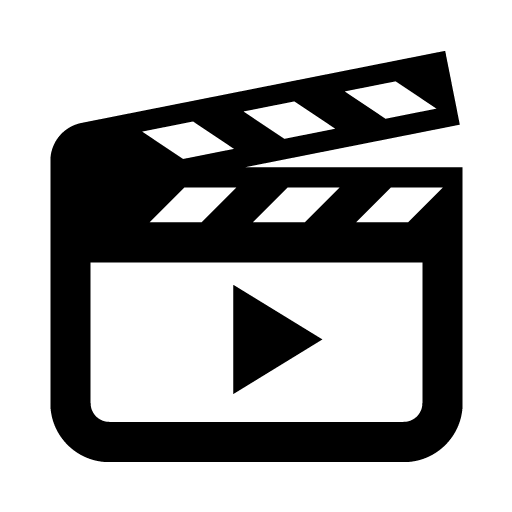
\includegraphics[width=0.10\textwidth]{05.IyA.imagenes/Video.png}}


\end{frame}

\begin{frame}{Errores br\'ujula magn\'etica. Giro}


  \begin{center}
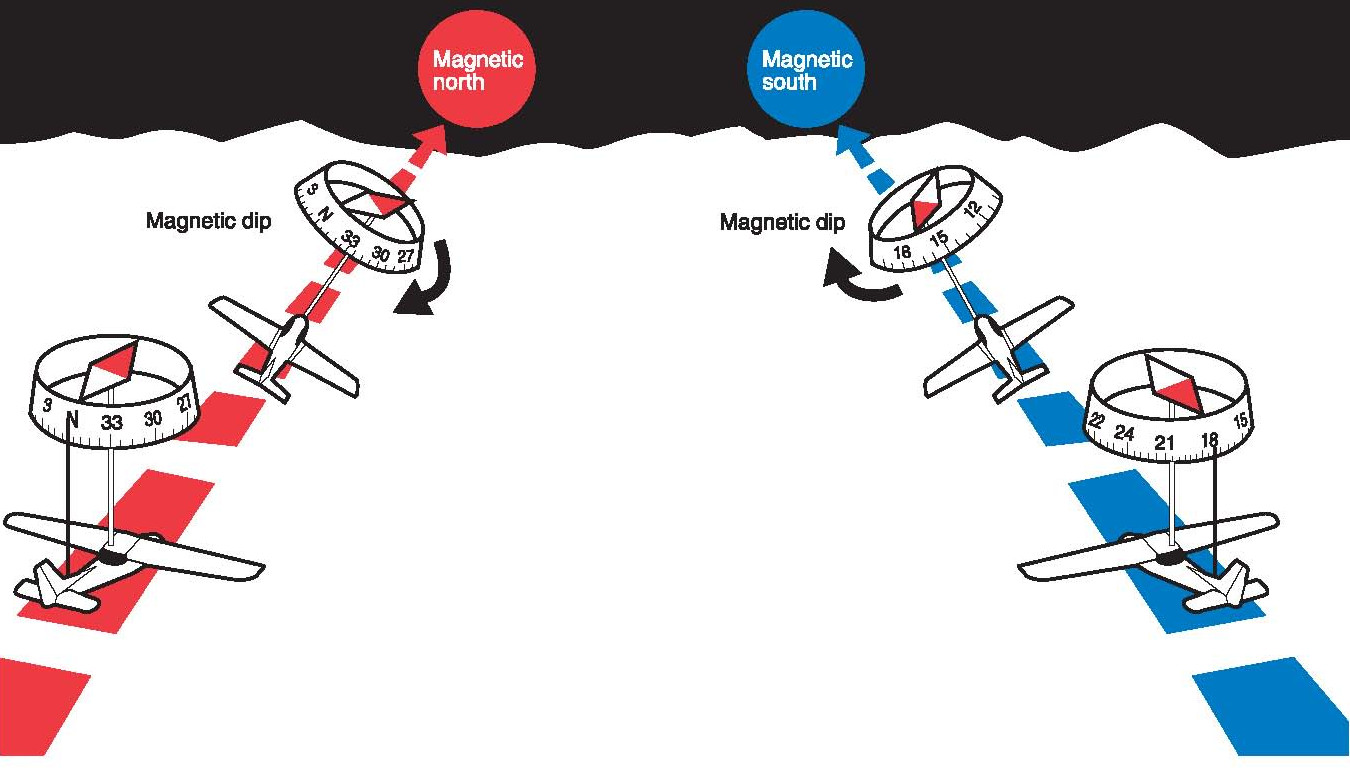
\includegraphics[width=0.80\textwidth]{05.instrumentos.giroscopicos.imagenes/05.04.MagnetismoTerrestre/05-04-brujula_error_giro.jpg}
\end{center}
  
  
\href{https://www.youtube.com/watch?v=WqXujnDw-kE}{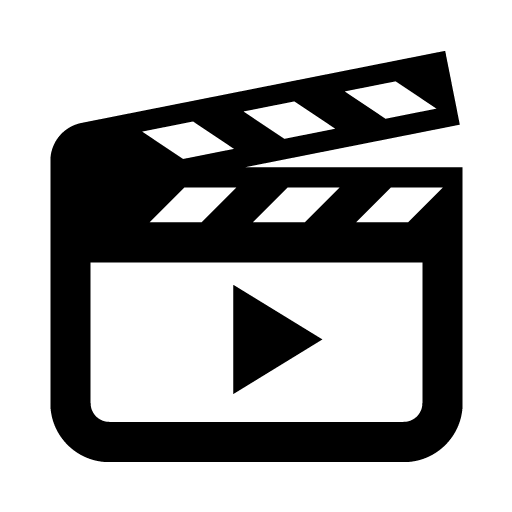
\includegraphics[width=0.10\textwidth]{05.IyA.imagenes/Video.png}}

\end{frame}

% 5.5.      Compás giroscópico auto-corregido, indicador con giróscopo integrado, y remoto.
% version 2019

\section{Comp\'as girosc\'opico auto-corregido, indicador con gir\'oscopo integrado, y remoto.}
\label{sec:compas.giroscopico.autocorregido}

\subsection{Comp\'as girosc\'opico auto-corregido}
\label{sec:compas.giroscopico.autocorregido}

\begin{frame}{Directional Gyro Indicator}

El Directional Gyro Indicator (DGI) o Direction Indicator (DI) es un
instrumento que consiste en un gir\'oscopo compuesto por una masa que
gira r\'apidamente, libre para moverse sobre uno o dos ejes, perpendicular
a los ejes de rotaci\'on y el uno de otro. Es una br\'ujula que mira siempre al
polo geogr\'afico.

El girocompás fue patentado en 1885 por el holand\'es Martinus Gerardus Van Den Bos, 
si bien su dise\~no nunca funcion\'o adecuadamente. En 1889, el capit\'an Arthur Krebs 
dise\~n\'o un gir\'oscopo pendular el\'ectrico para el submarino experimental franc\'es Gymnote, 
que le permitir\'ia forzar un bloqueo naval en 1890. 

A principios del siglo XX, un problema militar importante fue el control y
la navegaci\'on de los barcos, que cada vez presentaban dise\~nos maas
avanzados. Entre los primeros avances a este respecto destac o el dise\~no
de sensores que posibilitaran el control en lazo cerrado.

En 1903 el alem\'an Herman Ansch\"utz-Kaempfe construy\'o un girocomp\'as
que funcionaba y obtuvo una patente sobre su dise\~no, en 1908 junto al estadounidense 
Elmer Ambrose Sperry patentaron el
instrumento en los Estados Unidos y Gran Breta\~na.

\end{frame}

% \begin{frame}
%   Para la Primera Guerra Mundial, Sperry quiso vender el invento a los alemanes y 
%   Ansch\"utz-Kaempfe 
% le denunci\'o por violaci\'on de patente. Sperry argument\'o que la patente de Ansch\"utz-Kaempfe 
% no era v\'alida 
% debido a que no mejoraba significativamente la anterior patente de van den Bos. 
% Este hecho marc\'o el inicio de una pugna legal
% por violaci\'on de patente entre ambos,
% se concluy\'o que Sperry la había infringido al usar un m\'etodo espec\'ifico de amortiguamiento, 
% Ansch\"utz-Kaempfe 
% gan\'o el caso en 1915.

% A partir de entonces el girocomp\'as fu\'e empleado para controlar la direcci\'on de los 
% barcos. 

% Fu\'e tambi\'en significativo el aporte de N. Minosrsky (1922), quien introdujo su controlador
% de tres t\'erminos para posibilitar el control de la direcci\'on, y emple\'o por primera vez
% el Proportional-Integral-Derivativo (PID) y consider\'o efectos no lineales en los
% sistemas de lazo cerrado.


% \end{frame}


\begin{frame}
  \begin{exampleblock}
    {Los DGI tienen las siguientes ventajas sobre la br\'ulula
    magn\'etica:}
	{
    \begin{itemize}
    \item Pueden se\~nalar el norte geogr\'afico, esto es el eje de
      giro del planeta Tierra
    \item No se ven afectados por acumulaciones de metal, como el
      casco de barcos y aeronaves
    \end{itemize}
	}
  \end{exampleblock}

  \begin{alertblock}{Los DGI tienen las siguientes desventajas sobre la br\'ulula
    magn\'etica:}
    {
      \begin{itemize}
      \item     Requieren de una fuente constante de energ\'ia.
      \item Son mucho m\'as costosos
      \end{itemize}
	}
  \end{alertblock}

\end{frame}

\begin{frame}{DGI. Desviaciones}

  \begin{itemize}
  	\item {\bf Desv\'io o precesi\'on real:} la fricci\'on de los rodamientos sobre los
que giran el motor y las cunas puede originar, con el tiempo,
desequilibrios de las cunas, lo que ocasiona desv\'ios del sistema
card\'anico, los cuales resultan pr\'acticamente inapreciables.

	\item {\bf Desv\'io o precesi\'on aparente:} mientras el eje de rotaci\'on del
gir\'oscopo se halla apuntando al Norte, el movimiento de rotaci\'on de
la tierra provoca una desviaci\'on aparente del eje del rotor,
aproximadamente 15\grad/hora x sen(latitud) .
  \end{itemize}

\end{frame}


\begin{frame}{Girocomp\'as esclavo}
  
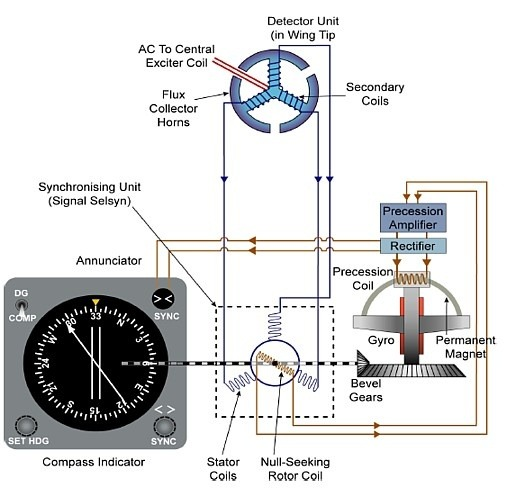
\includegraphics[width=0.7\textwidth]{05.instrumentos.giroscopicos.imagenes/05.05.DGI/05-05-girocompas_esclavo.jpg}

\end{frame}

% \begin{frame}{Girocomp\'as esclavo}

  

% \end{frame}




% \begin{frame}

%   {\tiny Ref: \url{https://www.ecured.cu/Br\%C3\%BAjula_girosc\%C3\%B3pica}}

% \end{frame}

% 5.6.      Central giroscópica para la indicación de actitud en tres ejes y toda actitud.

\section{Central girosc\'opica para la indicaci\'on de actitud en tres ejes y toda actitud}
\label{sec:central.giroscopica}

\subsection{Central girosc\'opica}
\label{sec:central.giroscopica.basico}

\begin{frame}
  
\end{frame}


\begin{frame}{AHRS}

\begin{block}{Attitude and Heading Reference Systems}
Los \textbf{Sistemas de Referencia de Actitud y Rumbo}, son sensores tridimensionales que proporcionan información acerca del rumbo, la actitud, y la guiñada de una aeronave. Este tipo de sistemas están específicamente diseñados para reemplazar a los antiguos instrumentos de control giroscópicos, y proporcionar una mejor precisión y fiabilidad. 

Est\'an conformados por gir\'oscopos o MEMs, acelerómetros, y magnetómetros, que proporcionan datos en los tres ejes del espacio. Algunos AHRS utilizan receptores GPS para mejorar la estabilidad a largo plazo de los giróscopos. Como técnica de fusión sensorial, es habitual emplear Filtros de Kalman, de tal manera que se obtenga una única solución a partir de las diversas fuentes de datos originales. Los AHRS se diferencian de los sistemas de navegación inercial en que se basan en el uso de magnetómetros y/o receptores GPS para corregir los datos en bruto (sin procesar) del giróscopo. 

\end{block}

\end{frame}


\begin{frame}{AHRS}

\begin{exampleblock}{Integraci\'on}
  Los AHRS se integran normalmente en Sistemas electrónicos de información de vuelo (EFIS)y se suelen combinar con Digital Air Data Computer (DADC), formando un Air Data, Attitude and Heading Reference Systems (ADAHRS), que proporciona información adicional tal como la velocidad del avión relativa al aire, altitud, y temperatura del aire en el exterior del avión. 
\end{exampleblock}

\begin{columns}
  \begin{column}{0.6\textwidth}
    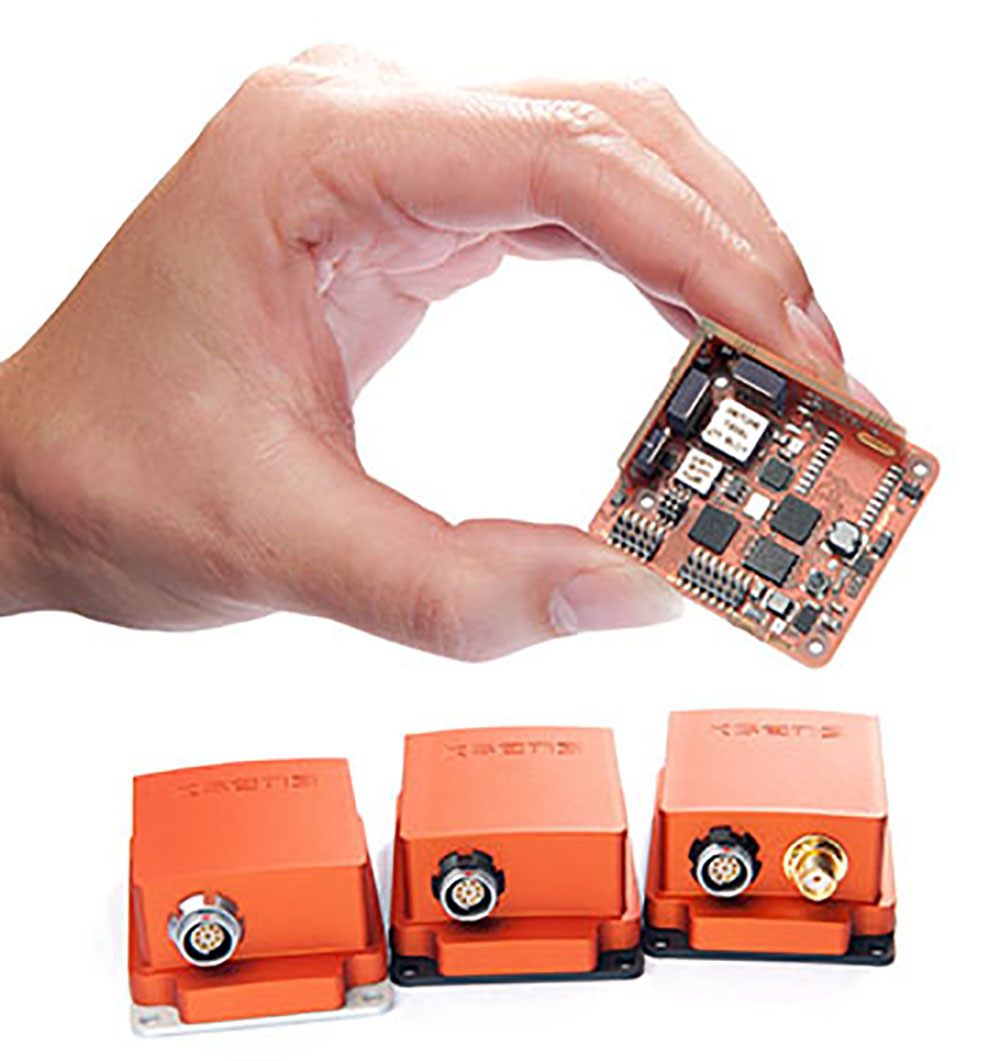
\includegraphics[height=0.45\textheight]{05.instrumentos.giroscopicos.imagenes/05.06.central.giroscopica/05-06-ahrs_.jpg}

    {\tiny Fuente: \url{https://www.xsens.com/products/mti-100-series/}}

\end{column}
\begin{column}{0.4\textwidth}
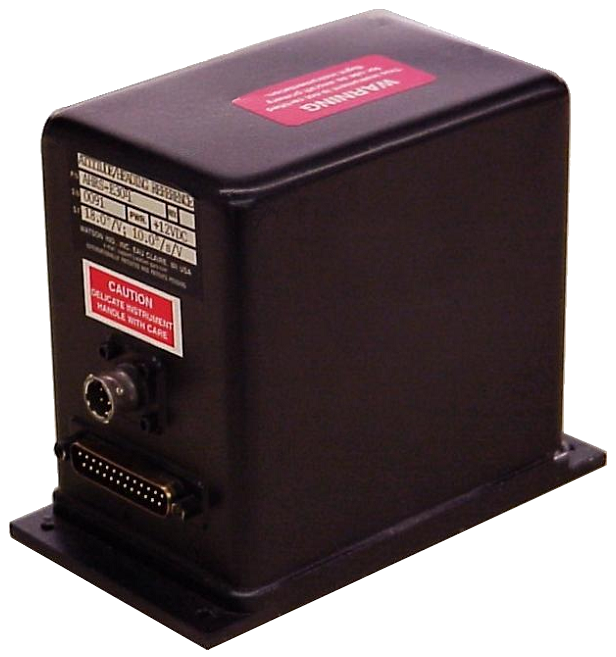
\includegraphics[height=0.45\textheight]{05.instrumentos.giroscopicos.imagenes/05.06.central.giroscopica/05-06-AHRS-E304_product.png}

      {\tiny Fuente: \url{https://watson-gyro.com/?s=ahrs} }

\end{column}
\end{columns}

\end{frame}

% \begin{frame}{AFCS}
  
%   \begin{block}{Automatic Flight Control System}
%     Es el sistema base de control de las futuras aeronaves no tripuladas, se basa en los siguientes conceptos:
%     \begin{itemize}
%     \item Equipar un piloto automático que controle la navegación
%     \item Enviar y recibir información de telemetría y comandos a/de la estación terrestre
%     \item Controlar los sistemas eléctrico, propulsivo y de presurización de la aeronave.
%     \end{itemize}
% Debe cumplir las siguientes funciones:
% \begin{itemize}
% \item Aceptar órdenes de la estación terrestre y realizar los comandos en la aeronave.
% \item  Monitorizar los subsistemas y detectar fallos.
% \item  Determinar altitud y posición y proveer de estos datos al piloto automático.
% \item  Seguir el algoritmo guía.
% \item  Poder retornar a casa en caso de emergencia. 
% \end{itemize}
%   \end{block}

% \end{frame}

% \begin{frame}

% 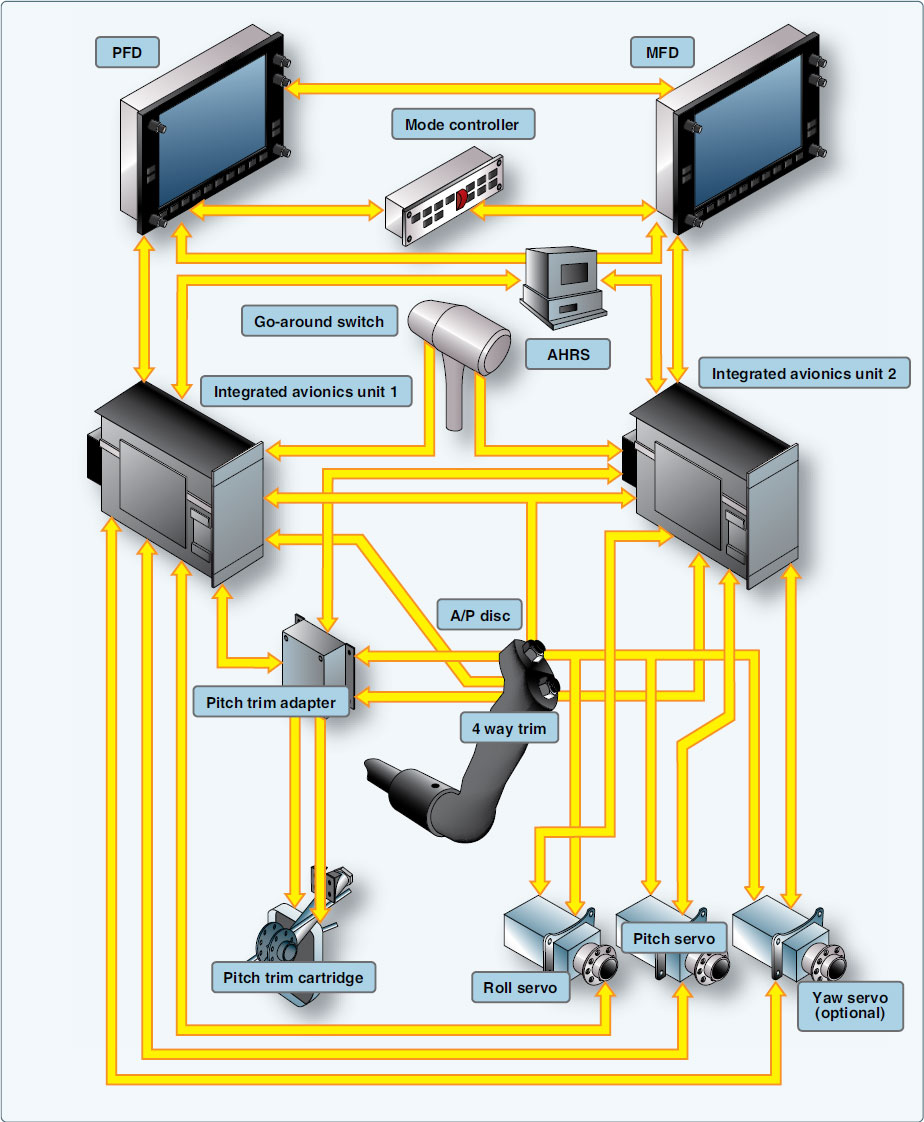
\includegraphics[height=0.85\textheight]{05.instrumentos.giroscopicos.imagenes/05.06.central.giroscopica/05-06-AFCS_0001.jpg}

% {\tiny Fuente: \url{https://www.flight-mechanic.com/automatic-flight-control-system-afcs-and-flight-director-systems/}}
% \end{frame}

%% 5.7.      Giróscopo LASER
% version 2019

\section{Gir\'oscopo Laser}
\label{sec:giroscopo.laser}

\begin{frame}
  
\end{frame}



%-----------------acronimos

% \section{Acr\'onimos}
% \label{sec:acronimos}

% %****** Acronyms and abbreviations in avionics ******
%***** [edit] A *****

% \acrodef{AGPL}{Affero General Public License}
% AGPL: Affero General Public License.




%     * ACARS: Aircraft Communications Addressing and Reporting System
%     * ACAS: Airborne Collision Avoidance System
%     * ACP: Audio control panel
%     * ACS: Audio control system
%     * ADAHRS: Air data and attitude heading reference system
%     * ADC: Air data computer
%     * ABAS: Aircraft-based augmentation system
%     * ADF: Automatic direction finder
%     * ADI: Attitude director indicator
%     * ADIRS: Air Data Inertial Reference System
%     * ADIRU: Air data inertial reference unit
%     * ADM: Air data module
%     * ADS: Either; Automatic Dependent Surveillance or air data system
%     * ADS-A: Automatic Dependent Surveillance-Address
%     * ADS-B: Automatic Dependent Surveillance-Broadcast
%     * AFCS: Automatic flight control system
%     * AFD: Autopilot flight director
%     * AFDC: Autopilot flight director computer
%     * AFDS: Autopilot flight director system
%     * AFIS: Either; Automatic flight information service or airborne flight
%       information system
%     * AGACS: Automatic ground–air communications system, is also known as ATCSS
%       or data link
%     * AGDL: Air-Ground Data Link
%     * AGC: Automatic gain control
%     * AHC: Attitude heading control
%     * AHRS: Attitude and Heading Reference Systems

\acrodef{AIDS}{Aircraft Integrated Data System}
      AIDS: Aircraft Integrated Data System

%     * ALC: Automatic level control
%     * ALT: Either; altimeter or altitude
%     * ALT Hold: altitude hold mode
%     * ALTS: Altitude select
%     * AMLCD: Active-matrix liquid crystal display
%     * ANC: Active noise cancellation
%     * ANN: Annunciator – caution warning system normally containing visual and
%       audio alerts to the pilot
%     * ANR: Active noise reduction
%     * ANT: Antenna
%     * A/P: Autopilot
%     * APC: Autopilot computer
%     * APS: Autopilot system
%     * APU: Auxiliary power unit
\acrodef{ARINC}{Aeronautical Radio INCorporated}
	ARINC: Aeronautical Radio INCorporated 

%     * ASD: Aircraft situation display
%     * ASDL: Aeronautical satellite data link
%     * ASR: Airport surveillance radar
%     * ASU: Avionics switching unit
\acrodef{ATC}{Air traffic control} ATC: Air traffic control
%     * ATCRBS: Air Traffic Control Radar Beacon System
%     * ATCSS: Air traffic control signaling system
%     * ATI: Unit of measure for instrument size, a standard 3¨û cutout is a 3ATI
%     * ATM: Air traffic management

\acrodef{ATSU}{Air Traffic Services Unit}
	ATSU: Air Traffic Services Unit%, implementada por AIRBUS en sus aviones (no en los A300/310), 
%		realiza las funciones generalmente usuales en unidades de gesti\'on de comunicaciones
%		de otro tipo de aviones.

%     * Avionics: Aviation + electronics
%     * AWG: American wire gauge


% ***** [edit] B *****
%     * B RNAV: Basic area navigation
%     * BARO: Barometric indication, setting or pressure
%     * BCRS: Back course
%     * BDI: Bearing distance indicator
%     * BGAN: Broadcast Global Area Network
\acrodef{BIT}{BInary Digit}
	BIT: BInary Digit

% ***** [edit] C *****
%     * CAI: Caution annunciator indicator
%     * CAT I: Operational performance Category 1
%     * CAT I Enhanced Allows for lower minimums than CAT I in some cases to CAT
%       2 minimums
%     * CAT II: Operational performance Category II
%     * CAT IIIa: Operational performance Category IIIa
%     * CAT IIIb: Operational performance Category IIIb
%     * CAT IIIc: Operational performance Category IIIc
%     * CODEC: Coder/decoder
%     * CDI: Course deviation indicator
%     * CDTI: Cockpit display of traffic information

\acrodef{CFDS}{Centralised Fault Display System}
	CFDS: Centralised Fault Display System

%     * CFIT: Controlled flight into terrain

\acrodef{CDU}{Control Display Unit}
	CDU: Control Display Unit

%     * COMM or COM: Communications receiver
%     * CNS: Communication, navigation, surveillance
%     * CNS/ATM: Communication, navigation, surveillance/air traffic Management
%       [1]
%     * CPDLC: Controller–pilot data link communications
%     * CPS: Cycles per second
%     * CRT: Cathode ray tube
\acrodef{CRT}{Cathode Ray Tube}
	CRT: Cathode Ray Tube
%     * CTAF: Common traffic advisory frequency
%     * CV/DFDR: Cockpit voice and digital flight data recorder
%     * CVR: Cockpit voice recorder
%     * CWS: Control wheel steering
% ***** [edit] D *****
%     * DA: Drift angle
%     * DAPs: Downlink of aircraft parameters
%     * DCDU: Data link control and display unit
%     * DG: Directional gyroscope
%     * DGPS: Differential global positioning system
%     * DH: Decision height
\acrodef{DITS}{Digital Information Transfer System}
	DITS: Digital Information Transfer System
%     * DLR: Data link recorder
%     * DME: Distance measuring equipment
%     * DNC: Direct noise canceling
%     * DP: Departure procedures
%     * DSP: Digital signal processing
%     * DUAT: Direct user access terminal
% ***** [edit] E *****
%     * EADI: Electronic attitude director indicator

\acrodef{EFD}{Electronic flight display}
      EFD: Electronic flight display

%     * EFIS: Electronic flight instrument system
%     * EGPWS: Enhanced ground proximity warning system
%     * EGT: Exhaust gas temperature
%     * EHS: Enhanced surveillance
%     * EHSI: Electronic horizontal situation indicator

\acrodef{EICAS}{Engine indication crew alerting system}
      EICAS: Engine indication crew alerting system

%     * ELT: Emergency locator transmitter
%     * ENC: Electronic noise canceling
%     * ENG: Engine
%     * ENR: Electronic noise reduction
%     * EPR: Engine pressure ratio
%     * ETOP: Extended-range twin-engine operation
% ***** [edit] F *****
%     * FADEC: Full authority digital engine control
%     * FANS: Future Air Navigation System
%     * FAT: Free air temperature
%     * FDPS: Flight plan Data Processing System
%     * FDRS: Flight data recorder system
%     * FDU: Flux detector unit
%     * FF: Fuel flow
%     * FIS-B: Flight information services – broadcast
%     * FLIR: Forward-looking infra-red
%     * FLTA: Forward-looking terrain avoidance

\acrodef{FMC}{Flight Management Computer}
	FMC: Flight Management Computer

\acrodef{FMGS}{Flight Management Guidance System}
	FMGS: Flight Management Guidance System

\acrodef{FMS}{Flight Management System}
      FMS: Flight Management System

%     * FREQ: Frequency
%     * FSS: Flight service station
%     * FWS: Flight warning system
%     * FYDS: Flight director/ Yaw damper system

% ***** [edit] G *****

%     * GBAS: Ground based augmentation system
%     * GCAS: Ground collision avoidance system
%     * GCU: Generator control unit
%     * GDOP: Geometric dilution of precision
%     * GGS: Global positioning system ground station
%     * GHz: Gigahertz
%     * GLNS: GPS Landing and Navigation System
%     * GLNU: GPS landing and navigation unit
%     * GLONASS: Global Navigation Satellite System
%     * GLS: GPS Landing System
%     * GLU: GPS landing unit

\acrodef{GND}{Ground}
	GND: Ground (tierra)


    % * GNSS: Global Navigation Satellite System
    % * GMT: Greenwich Mean Time

\acrodef{GPS}{Global Positioning Satellite or Global Positioning System}
    GPS: Global Positioning Satellite or Global Positioning System

    % * GPWC: Ground proximity warning computer

\acrodef{GPWS}{Ground proximity warning system}
     GPWS: Ground proximity warning system

% ***** [edit] H *****
%     * HDG: Heading
%     * HDG SEL: Heading select
%     * HDOP: Horizontal dilution of precision
%     * HF: High frequency
%     * HHLD: Heading hold
%     * HSD: High-speed data
%     * HSI: Horizontal situation indicator
%     * HSL: Heading select
%     * HUD: Head-up display
%     * HMD: Helmet-mounted display
% ***** [edit] I *****
%     * IAS: Indicated airspeed
%     * ID: Identify/Identification or identifier
%     * IDENT: Identify/identifier
%     * IDS: Information display system or integrated display system
%     * IFE: In-flight entertainment
%     * IFR: Instrument flight regulations
%     * ILS: Instrument landing system
%     * IMC: Instrument meteorological conditions
%     * InHg: Inch of Mercury
%     * IND: Indicator[disambiguation needed]
%     * INS: Inertial Navigation System
%     * ISA: International Standard Atmosphere
%     * ISP: Integrated switching panel
%     * ITT: Interstage turbine temperature
%     * IVSI: Instantaneous vertical speed indicator
% ***** [edit] J *****
%     * JTIDS: Joint Tactical Information Distribution System
% ***** [edit] L *****
%     * LAAS: Local Area Augmentation System
%     * LADGPS: Local Area Differential GPS
%     * LCD: Liquid crystal display
\acrodef{LCD}{Liquid Crystal Display}
	LCD: Liquid Crystal Display

%     * LDGPS: Local area differential global positioning satellite
%     * LED: Light-emitting diode
%     * LMM: Locator middle marker
%     * LOC: Localizer
%     * LOM: Locator outer marker
%     * LORAN: Long-range navigation
%     * LRU: Line-replaceable unit
% ***** [edit] M *****
%     * MAP: Manifold absolute pressure or missed approach point
%     * MB: Marker beacon
%     * MCBF: Mean cycles between failures

\acrodef{MCDU}{Multi Control Display Unit}
	MCDU: Multi Control Display Unit

%     * MDA: Minimum decent altitude
%     * MEL: Minimum equipment list
%     * MF: Medium frequency
%     * MFD: Multi-function display
%     * MFDS: Multi-function display system
%     * MIC: Microphone
%     * MIDS: Multifunctional information distribution system
%     * MILSPEC: Military specification
%     * MKR: Marker beacon
%     * MLS: Microwave landing system
%     * MM: Middle marker
%     * MNPS: [Minimmum navigation performance specifications]
%     * MMD: Moving map display
%     * MOA: Military operations area
%     * Mode A: Transponder pulse-code reporting
%     * Mode C: Transponder code and altitude reporting
%     * Mode S: Transponder code, altitude, and TCAS reporting
%     * MOSArt: Modular Open System Architecture
%     * MSG: Message
%     * MSP: Modes S-Specific Protocol
%     * MSSS: Mode S-Specific Services
%     * MTBF: Mean time between failures
%     * MTTF: Mean time to failure


%     * MVFR: Marginal visual flight rules
% ***** [edit] N *****
%     * NAS: National Airspace System
%     * NAV: Navigation receiver
%     * Navaid: Navigational aid
%     * NAVCOMM: Navigation and communications equipment or receiver
%     * NAVSTAR-GPS: The formal name for the space-borne or satellite navigation
%       system
%     * NCATT: National Center for Aircraft Technician Training
%     * ND: Navigation display
%     * NDB: Non-directional radio beacon
%     * NFF: No fault found
%     * NM or NMI: Nautical mile
%     * NoTAM: Notice to airmen
%     * NPA: Non-precision approach
%     * NVD: Night vision device
%     * NVG: Night vision goggles

% ***** [edit] O *****
%     * OAT: Outside air temperature
%     * OBS: Omnibearing selector
%     * OM: Outer marker
\acrodef{OLED}{Organic Light-Emitting Diode}
	OLED: Organic Light-Emitting Diode

% ***** [edit] P *****
%     * PA: Public address system
%     * P-Code: GPS precision code
%     * PAPI: Precision approach path indicator
%     * PAR: Precision approach radar
%     * PD: Profile descent
%     * PDOP: Position dilution of precision
%     * PFD: Primary flight display or primary flight director
%     * PMG: Permanent magnet generator
%     * PND: Primary navigation display
%     * PNR: Passive noise reduction
%     * POS: Position[disambiguation needed]
%     * P-RNAV: precision area navigation
%     * PSR: Primary surveillance radar
%     * PTT: Push-to-talk
% ***** [edit] R *****
%     * RA: Resolution advisory (TCAS)
%     * RAI: Radio altimeter indicator
%     * RAIM: Receiver-autonomous integrity monitoring, also remote autonomous
%       integrity monitoring
%     * RALT: Radar or radio altimeter
%     * RAT: Ram air turbine
%     * RCR: Reverse current relay
%     * RCVR: Receiver
%     * RDMI: Radio distance magnetic indicator
%     * RDP: Radar data processing system
%     * RDR: Radar
%     * REF: Reference
%     * REIL: Runway end identifier lights
%     * REL: Relative[disambiguation needed]
%     * RF: Radio frequency
%     * RFI: Radio frequency interference
%     * RHSM: Reduced horizontal separation minimal
%     * RLG: Ring laser gyroscope
%     * RLY: Relay
%     * RMI: Radio magnetic indicator
%     * R-NAV: Area navigation
%     * RNG: Range
%     * RNP: Required navigation performance
%     * ROC: Rate of climb
%     * ROD: Rate of descent
%     * RPA: Remotely piloted aircraft (Unmanned aerial vehicle)
%     * RPM: Revolutions per minute
%     * RTE: Route
%     * RVR: Runway visual range
%     * RVSM: Reduced vertical separation minimum
%     * RX: Receiver
% ***** [edit] S *****
%     * SAT: Static air temperature
%     * SATCOM: Satellite communication
%     * SATNAV: Satellite navigation
%     * SD: Secure digital
%     * SELCAL: Selective calling

\acrodef{SID}{Standard Instrument Departure}
      SID: Standard Instrument Departure

%     * SIU: Satellite interface unit
%     * S: Sensitivity Level
%     * SMS: Short Messaging Service
%     * SNR: Signal-to-noise ratio
%     * SPKR: Speaker
%     * SQ or SQL: Squelch
%     * SSCV/DR: Solid-state cockpit voice/data recorder
%     * SSCVR: Solid-state cockpit voice recorder
%     * SSFDR: Solid-state flight data recorder
%     * SSR: Secondary surveillance radar

\acrodef{STAR}{Standard Terminal Arrival Route}
      STAR: Standard Terminal Arrival Route

\acrodef{STARS}{Standard Terminal Automation Replacement System}
     STARS: Standard Terminal Automation Replacement System



%     * STC: Supplemental Type Certificate
%     * STCA: Short-Term Conflict Alert
%     * STP: Standard temperature and pressure
%     * SUA: Special use airspace
% ***** [edit] T *****
%     * TA: Traffic advisory (see TCAS)
%     * TACAN: Tactical air navigation system
%     * Tach: Tachometer
%     * TAD: Terrain awareness display
%     * TAF: Terminal area forecast
%     * TAS: True airspeed
%     * TAT: True air temperature, or total air temperature
%     * TAWS: Terrain awareness warning system
%     * TBO: Time before overhaul, or time between overhaul
%     * TCA: Throttle control assembly, or terminal control area
%     * TCAS: Traffic collision avoidance system
%     * TCF: Terrain clearance floor
%     * TCN: TACAN
%     * TCU: TACAN control unit
%     * TDOP: Time dilution of precision
%     * TDR: Transponder (in some cases)
%     * TERPS]]: Terminal instrument procedures, or terminal enroute procedures
%     * TFR: Temporary flight restrictions
%     * TFT: Thin-film transistor
%     * TGT: Turbine gas temperature, or target
%     * THDG: True heading
%     * TIAS: True indicated airspeed
%     * TIS: Traffic information service
%     * TK: Track angle
%     * TKE: Track-angle error
%     * TLA: Three-letter acronym
%     * TOGA: Takeoff/Go-around switch, Takeoff/go-around thrust
%     * TOT: Turbine outlet temperature
%     * TR or T/R: Transmitter receiver or transceiver
%     * TRACON: Terminal radar approach control
%     * TRANS: Transmit, Transmission, or Transition[disambiguation needed]
%     * TRK: Track
%     * TRP: Mode S transponder
%     * TTR: TCAS II transmitter/receiver
%     * TTS: Time to station
%     * TVE: Total vertical error
%     * TWDL: Two-way data link, or terminal weather data link
%     * TWDR: Terminal Doppler Weather Radar
%     * TWIP: Terminal weather information for pilots
%     * TWR: Terminal weather radar
%     * TX: Transmit
% ***** [edit] U *****
%     * UART: Universal asynchronous receiver transmitter
%     * UAV: Unmanned aerial vehicle
%     * UHF: Ultra-high frequency
%     * ULB: Underwater locator beacon
%     * USB: Universal Serial Bus
%     * UTC: Universal Time Coordinate
% ***** [edit] V *****
%     * V: Volts or voltage
%     * VASI: Visual approach slope indicator
%     * VDL: VHF Data Link
%     * VDR: VHF digital radio
%     * VFO: Variable frequency oscillator
%     * VFR: Visual flight rules
%     * VG/DG: Vertical gyroscope/directional gyroscope
%     * VGA: Video Graphics Array
%     * VHF: Very high frequency
%     * V/L: VOR/Localizer
%     * VMC: Visual meteorological conditions or minimum control speed with
%       critical engine out
%     * V/NAV: Vertical navigation
%     * VNE: Never exceed speed
%     * VNO: Maximum structural cruising speed
%     * VNR: VHF navigation receiver
%     * VOR: VHF omnidirectional range and ranging
%     * VOR/DME: VOR with Distance measuring equipment
%     * VOR/MB: VOR marker beacon
%     * VORTAC: VOR and TACAN combination
%     * VOX: Voice transmission
%     * VPATH: Vertical path
%     * V/R: Voltage regulator
%     * V/REF: Reference velocity
%     * V/S: Vertical speed
%     * VSI: Vertical speed indicator
%     * VSM: Vertical separation limit
%     * VSO: Stall speed in landing configuration
%     * VSWR: Voltage–standing wave ratio
%     * V/TRK: Vertical track
%     * VX: Speed for best angle of climb
%     * VY: Speed for best rate of climb
% ***** [edit] W *****
%     * WAAS: Wide Area Augmentation System
%     * WD/WINDR: Wind direction
%     * WMA: WXR waveguide adapter
%     * WMI: WXR indicator mount
%     * WMS: Wide-area master station
%     * WMSC: Weather message switching center
%     * WMSCR: Weather message switching center replacement
%     * WPT: Waypoint
%     * WRT: WXR receiver transmitter
%     * WX: Weather
%     * WXR: Weather radar system
%     * WYPT: Waypoint
% ***** [edit] X *****
%     * XCVR: Transceiver
%     * XFR: Transfer
%     * XMIT: Transmit
%     * XMSN: Transmission
%     * XMTR: Transmitter
%     * XPDR: Transponder
%     * XTK: Crosstrack
% ***** [edit] Y *****
%     * YD: Yaw damper
% ***** [edit] See also *****
%     * Avionics
%     * List of aviation, aerospace and aeronautical abbreviations
% ***** [edit] References *****
%    1. ^ http://wwwicaoint/icao/en/ro/rio/execsumpdf


% Retrieved from "http://en.wikipedia.org/w/
% index.php?title=Acronyms and abbreviations in avionics&amp;oldid=518531528"

% \addcontentsline{toc}{chapter}{Lista de Acr\'onimos}


%-------------Bibliografia
 \begin{frame}{Bibliograf\'ia}
   \bibliographystyle{apalike} 
   \bibliography{../IyA}
 \end{frame}


\end{document}
